% META: DONE.1

\chapterappendix{ПРИЛОЖЕНИЕ}{Г}

\begin{center}
{\fontseries{sb}\selectfont Примеры работы модуля}
\end{center}

В приложении приведены результаты обработки пяти типовых деталей. Для каждой детали указаны операции, использованные в оригинальном построении, использованные конфигурации нейронных сетей, и результаты классификации и визуализации сегментации.

\subsection{Деталь 01}

\begin{itemize}
    \item \textbf{Операции исходного построения:} bossExtrusion, fillet, chamfer.
    \item \textbf{Использованные конфигурации нейронных сетей:} классификация - B, сегментация - E.
    \item \textbf{Результат классификации:} fillet - 0.999\%, cutExtrusion - 0.255\%, chamfer - 0.736\%.
\end{itemize}

Результаты сегментации представлены на рисунке \ref{fig:part-01}.

\begin{figure}[h]
    \centering
    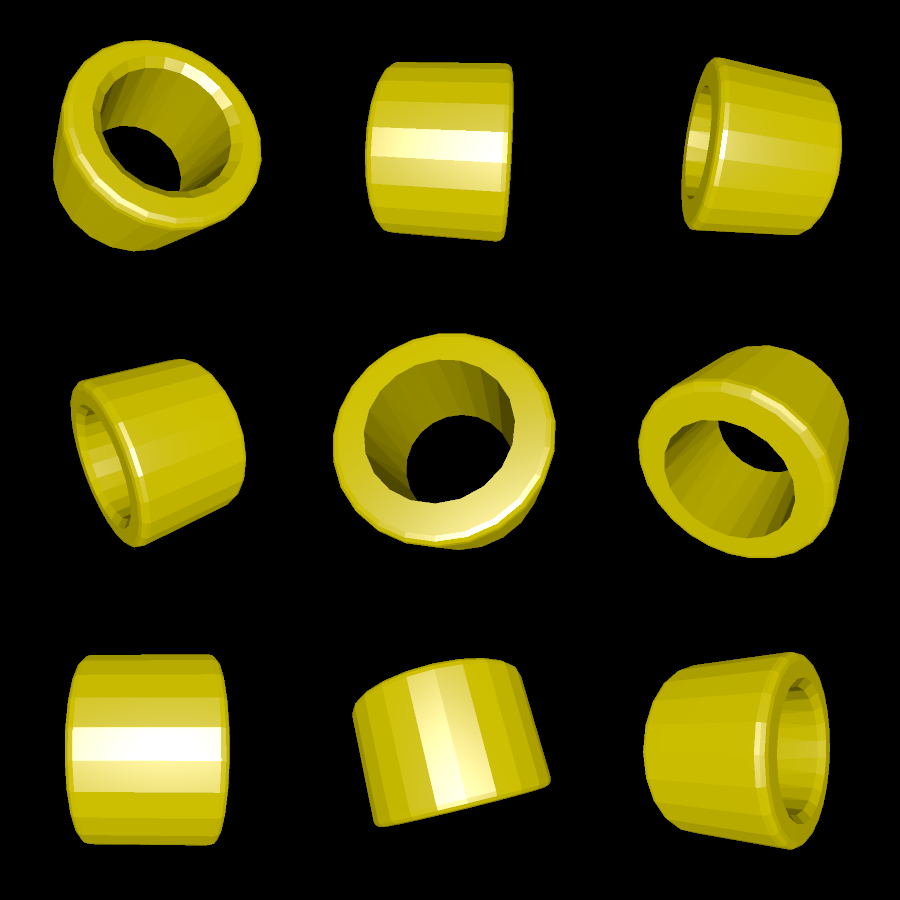
\includegraphics[width=0.3\linewidth]{figures/part_01_original.png}
    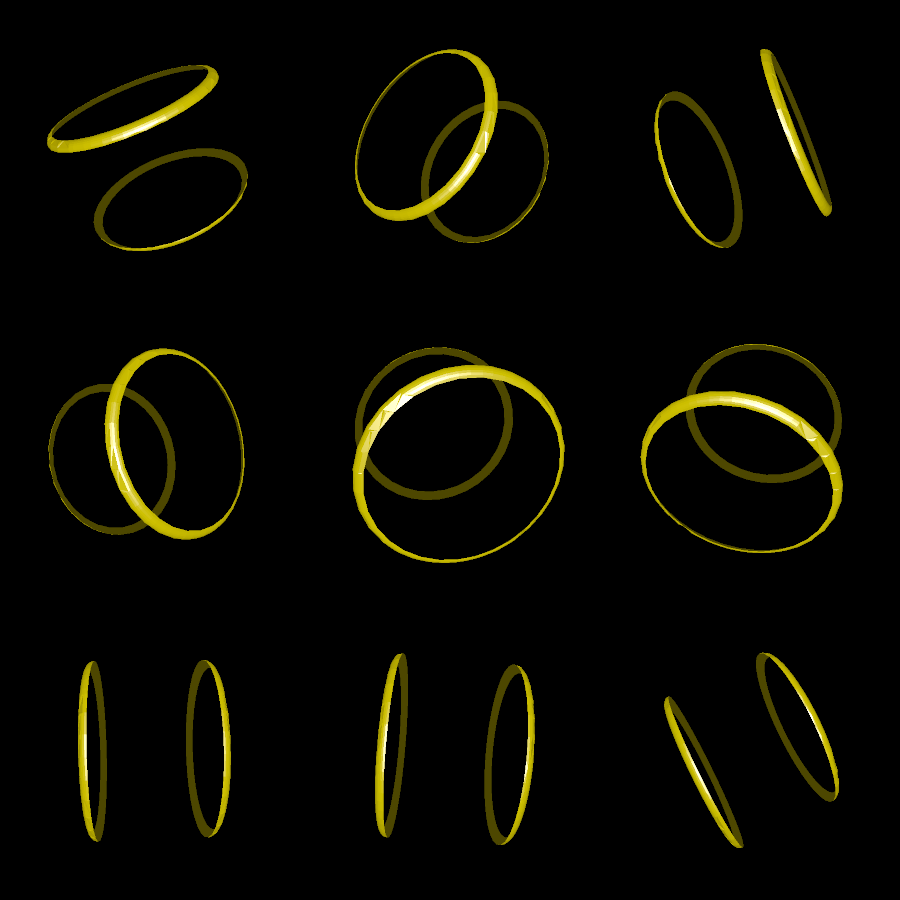
\includegraphics[width=0.3\linewidth]{figures/part_01_fillet_detected.png}
    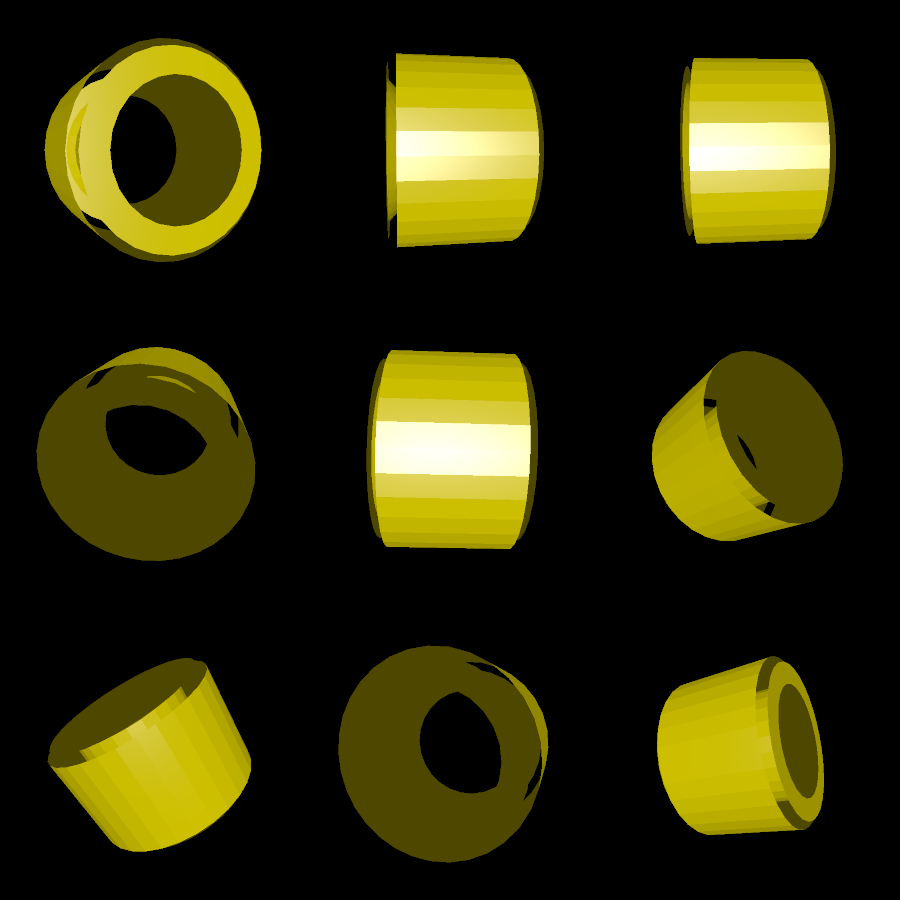
\includegraphics[width=0.3\linewidth]{figures/part_01_fillet_remaining.png} \\
    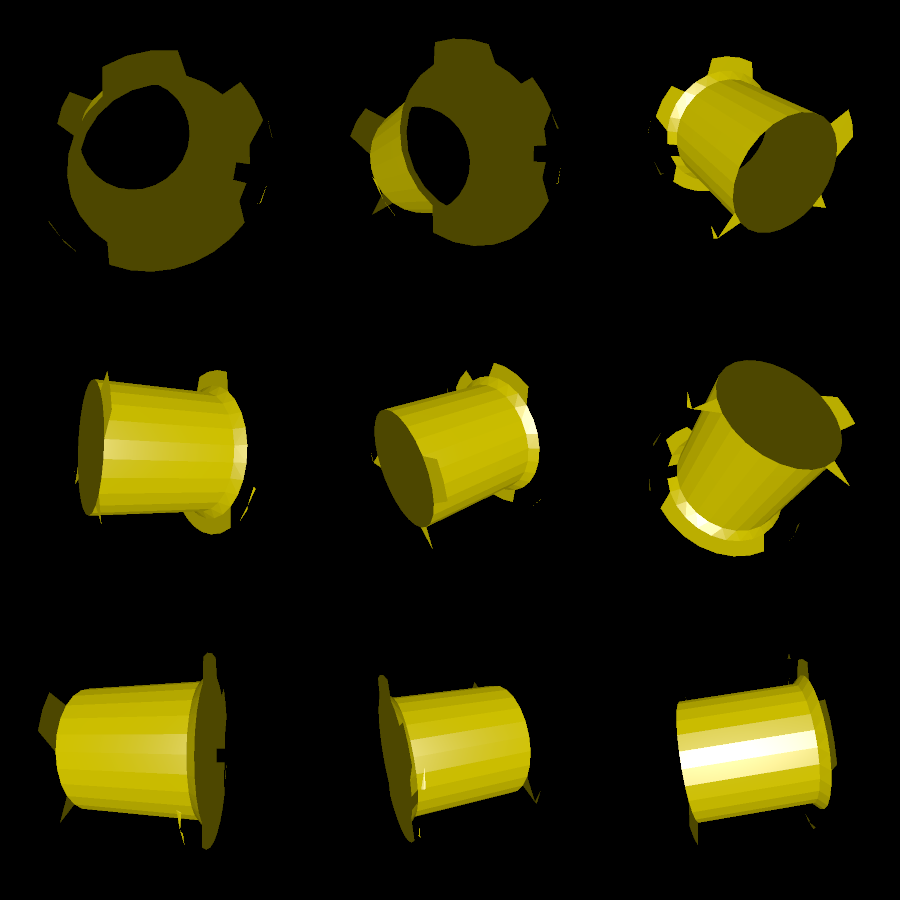
\includegraphics[width=0.3\linewidth]{figures/part_01_cutextrusion_detected.png}
    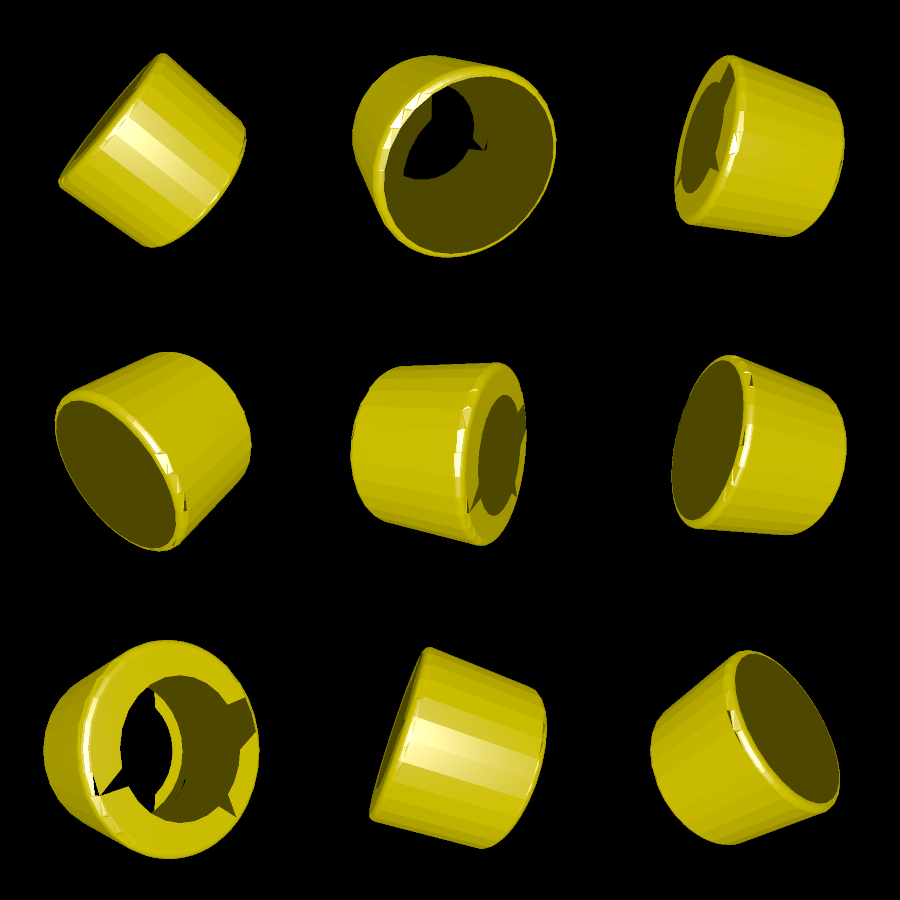
\includegraphics[width=0.3\linewidth]{figures/part_01_cutextrusion_remaining.png}
    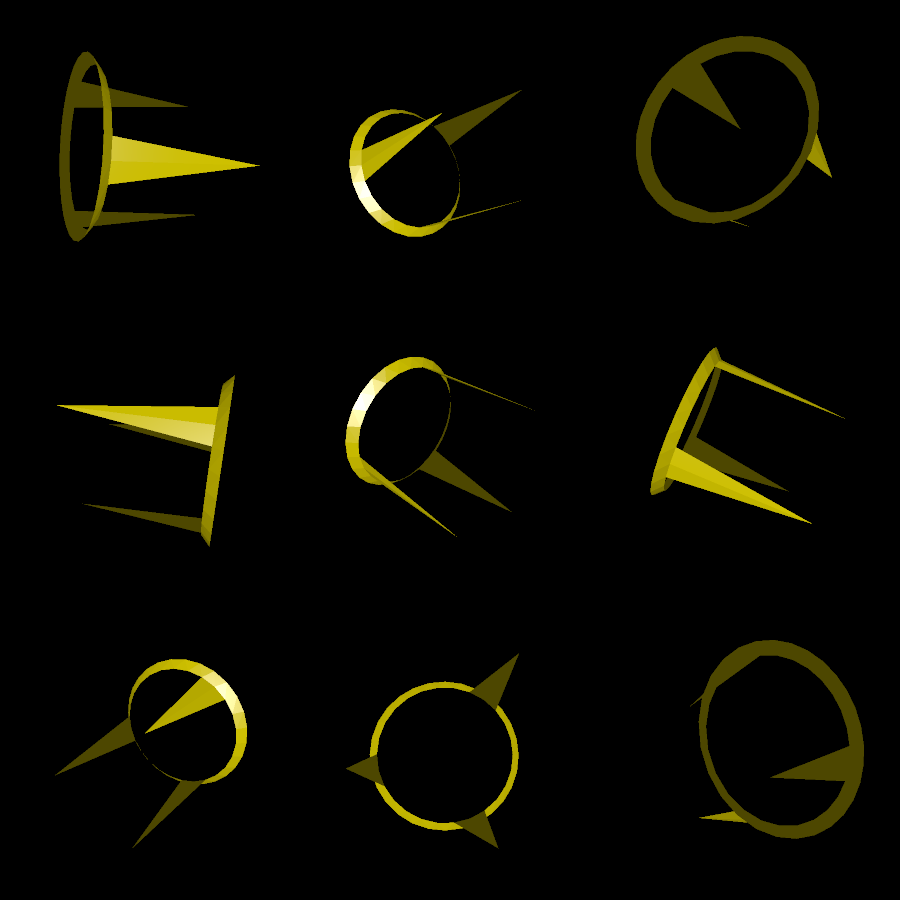
\includegraphics[width=0.3\linewidth]{figures/part_01_chamfer_detected.png} \\
    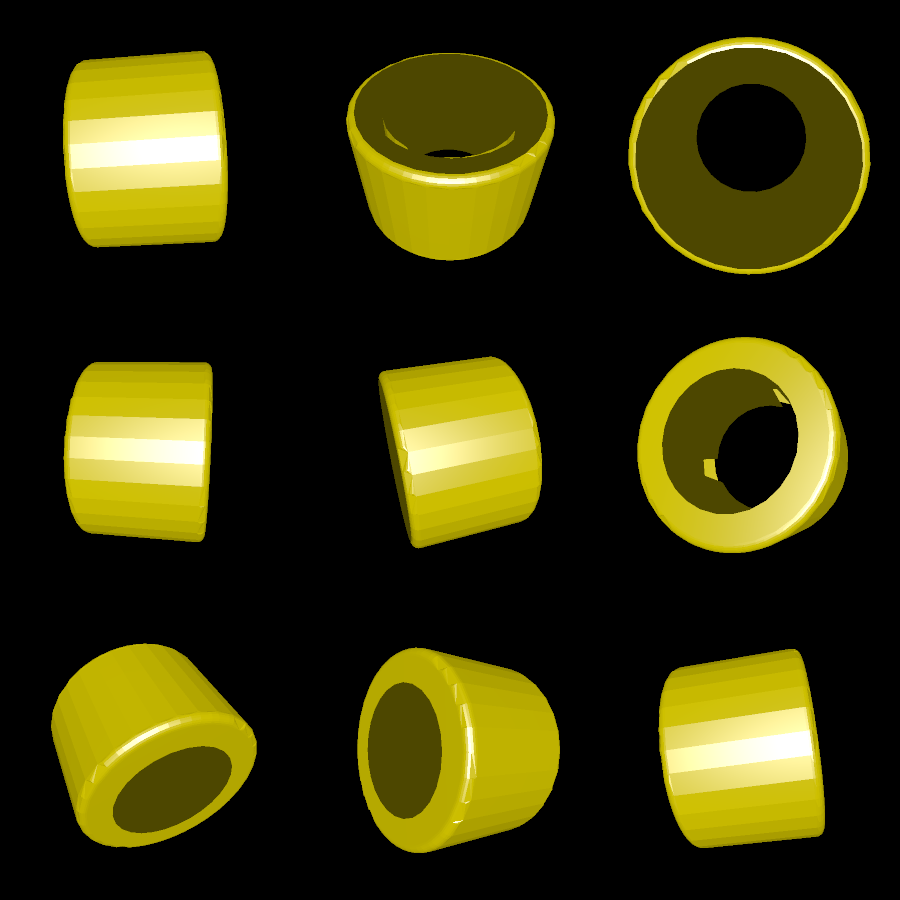
\includegraphics[width=0.3\linewidth]{figures/part_01_chamfer_remaining.png}
    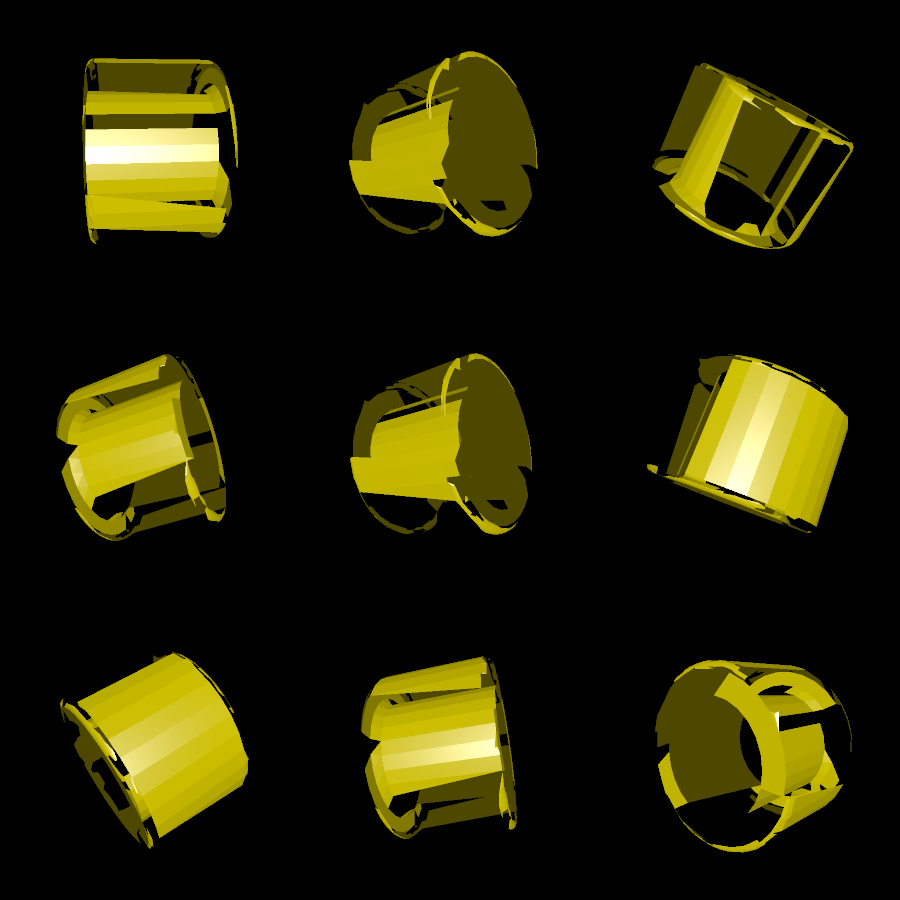
\includegraphics[width=0.3\linewidth]{figures/part_01_bossextrusion_detected.png}
    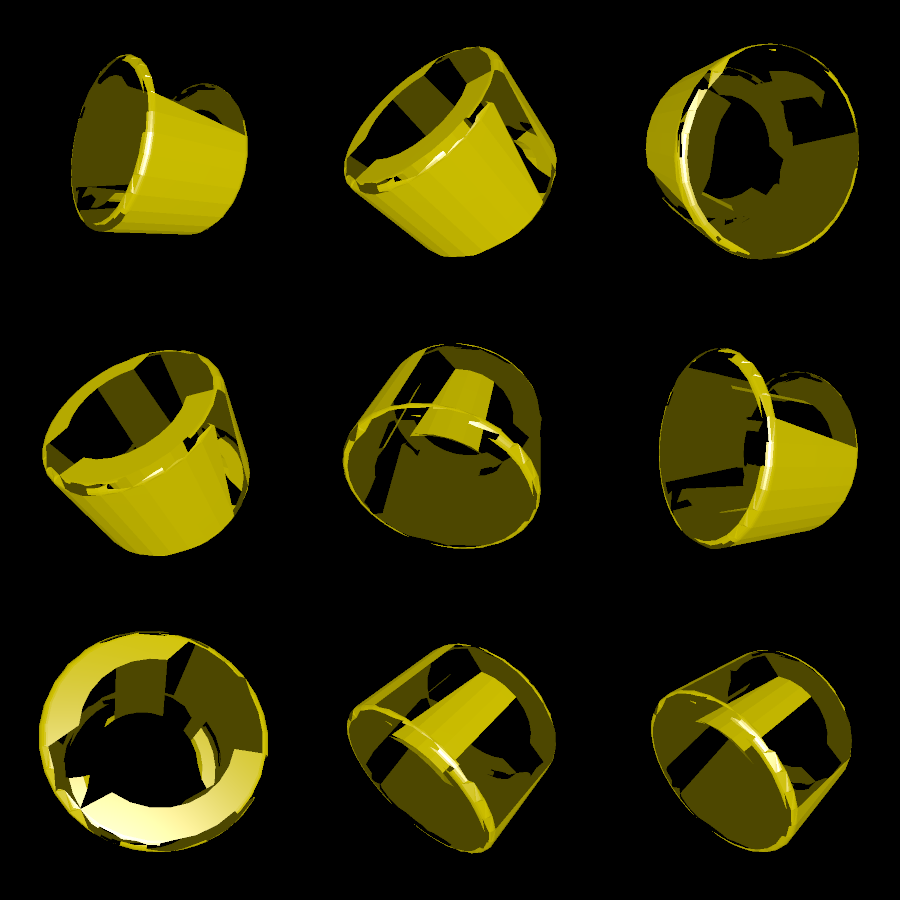
\includegraphics[width=0.3\linewidth]{figures/part_01_bossextrusion_remaining.png}
    \caption{Пример работы модуля на детали «Деталь 01», слева направо, сверху вниз: 1) исходная модель, 2) обнаруженная часть (fillet), 3) оставшаяся геометрия (fillet), 4) обнаруженная часть (cutExtrusion), 5) оставшаяся геометрия (cutExtrusion), 6) обнаруженная часть (chamfer), 7) оставшаяся геометрия (chamfer), 8) обнаруженная часть (bossExtrusion), 9) оставшаяся геометрия (bossExtrusion)}
    \label{fig:part-01}
\end{figure}

\subsection{Деталь 02}

\begin{itemize}
    \item \textbf{Операции исходного построения:} bossExtrusion, bossExtrusion, cutRotated, chamfer, cutRotated, cutExtrusion.
    \item \textbf{Использованные конфигурации нейронных сетей:} классификация - B, сегментация - E.
    \item \textbf{Результат классификации:} fillet - 0.999\%, cutExtrusion - 0.159\%, chamfer - 0.911\%.
\end{itemize}

Результаты сегментации представлены на рисунке \ref{fig:part-02}.

\begin{figure}[h]
    \centering
    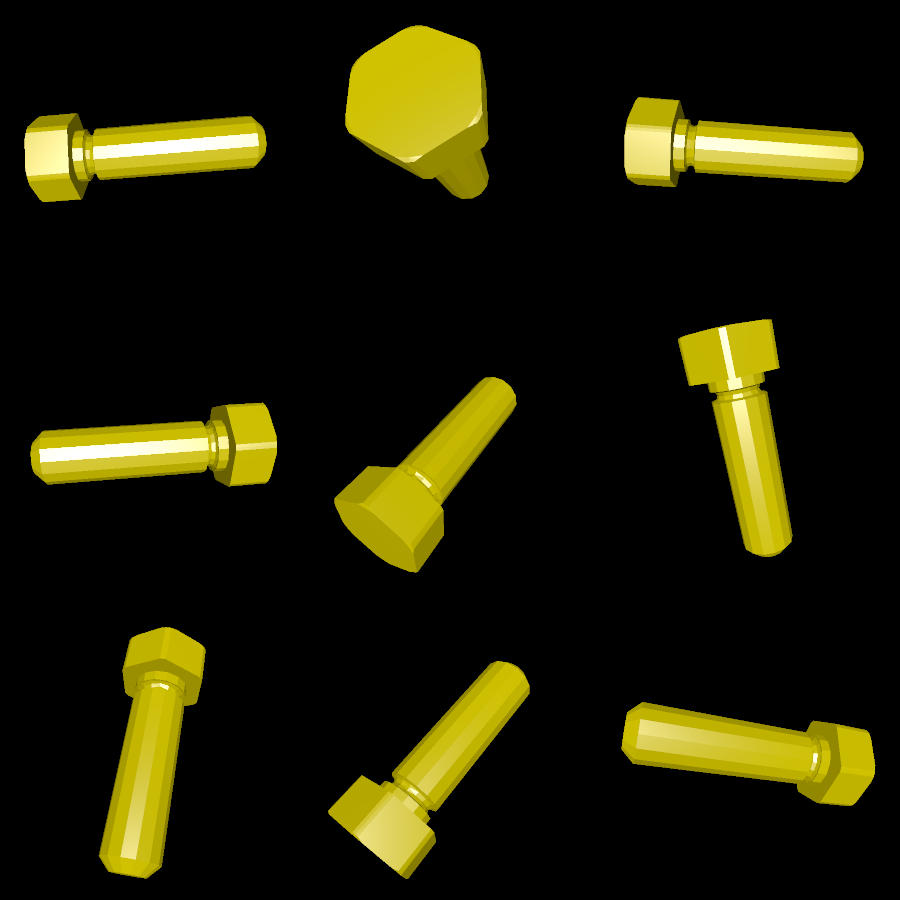
\includegraphics[width=0.3\linewidth]{figures/part_02_original.png}
    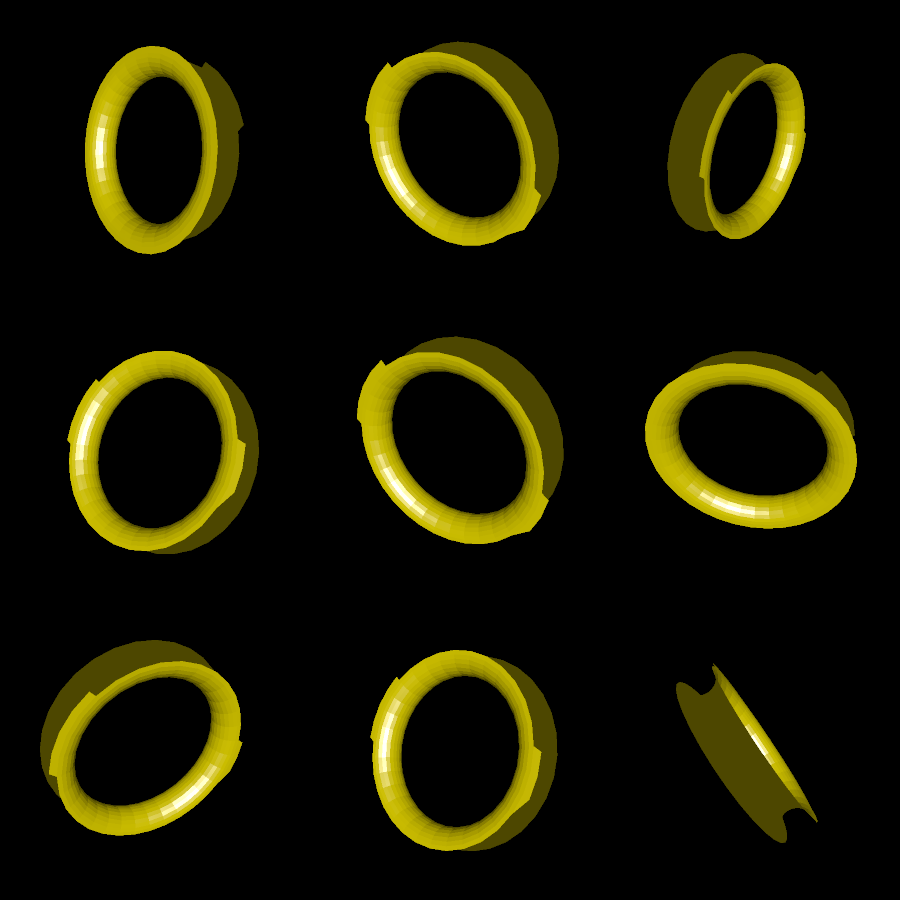
\includegraphics[width=0.3\linewidth]{figures/part_02_fillet_detected.png}
    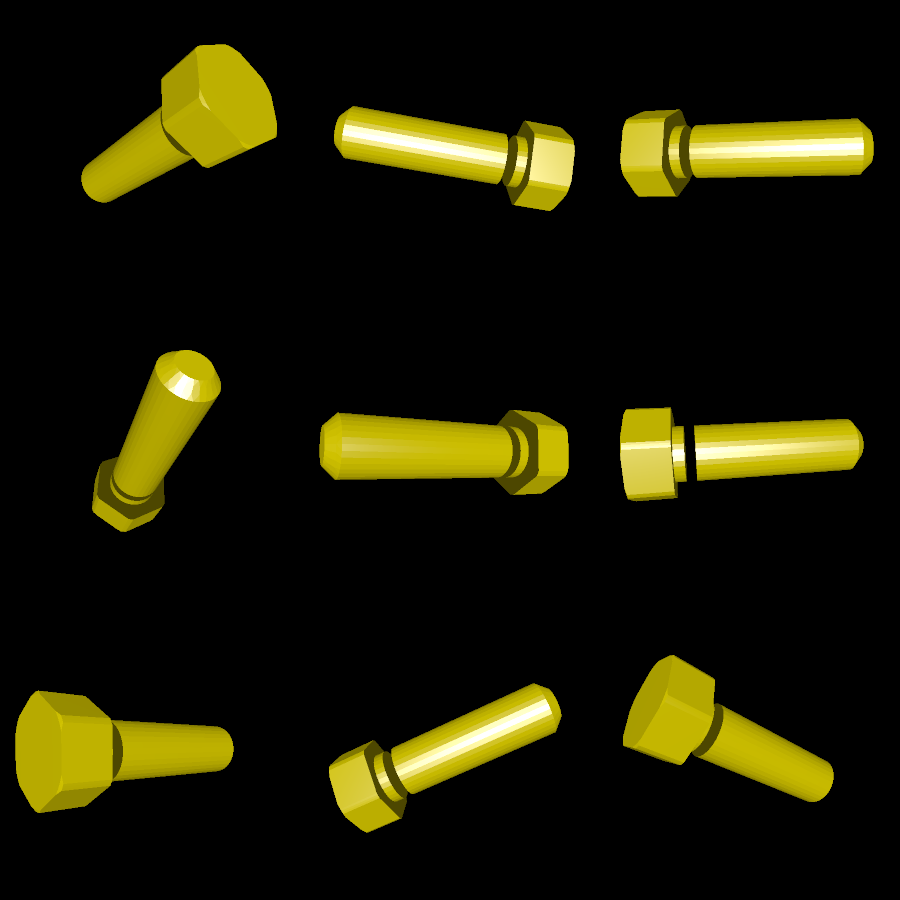
\includegraphics[width=0.3\linewidth]{figures/part_02_fillet_remaining.png} \\
    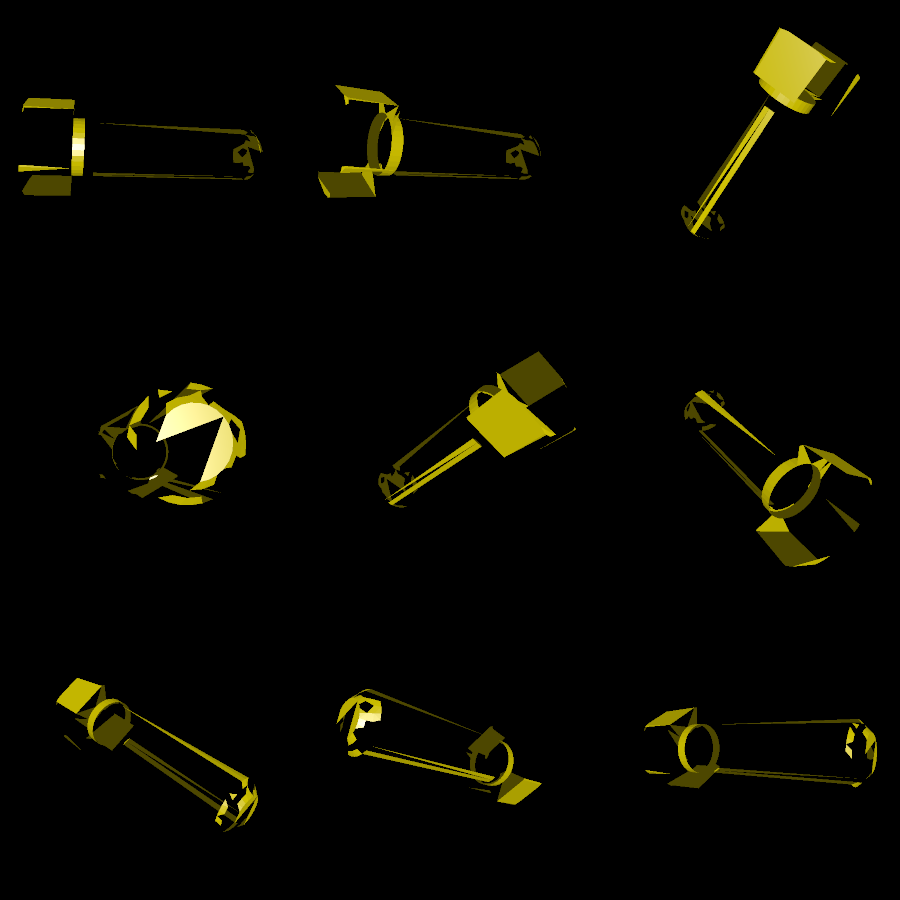
\includegraphics[width=0.3\linewidth]{figures/part_02_cutextrusion_detected.png}
    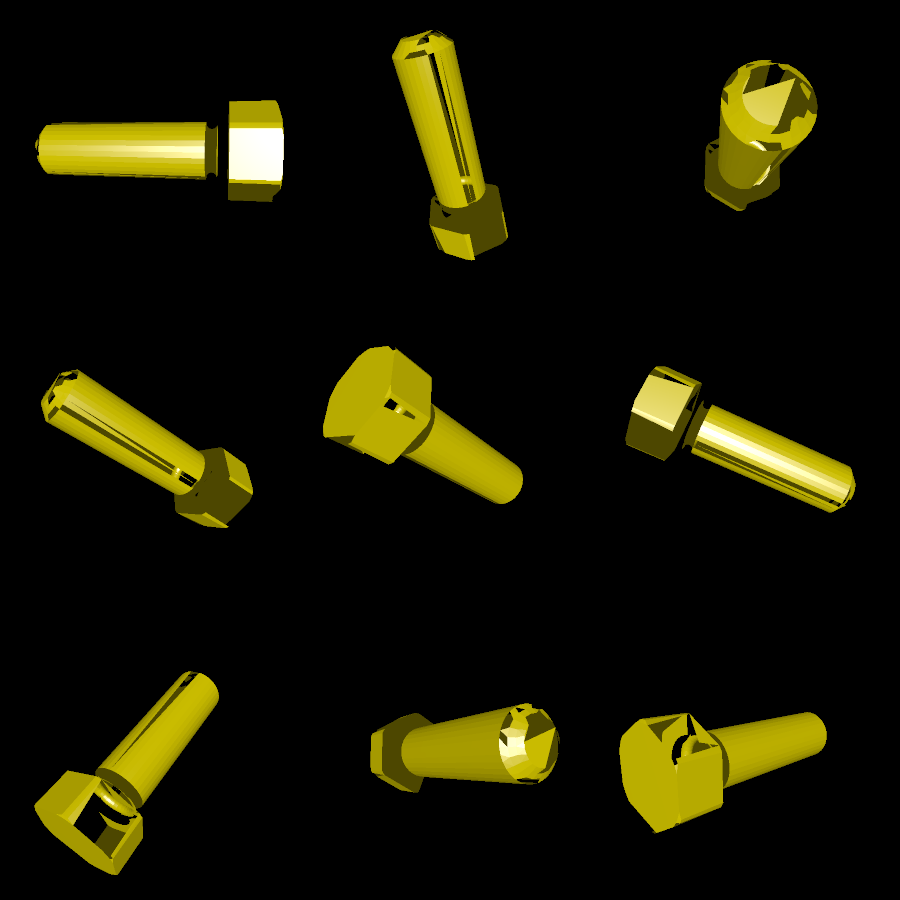
\includegraphics[width=0.3\linewidth]{figures/part_02_cutextrusion_remaining.png}
    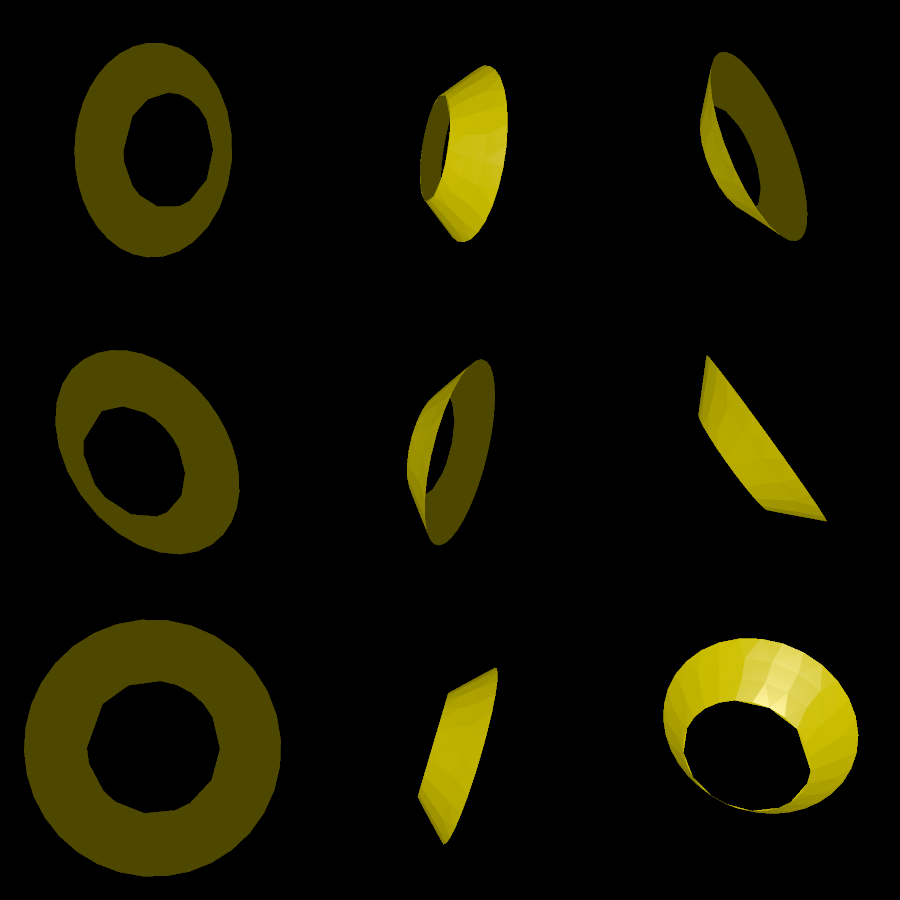
\includegraphics[width=0.3\linewidth]{figures/part_02_chamfer_detected.png} \\
    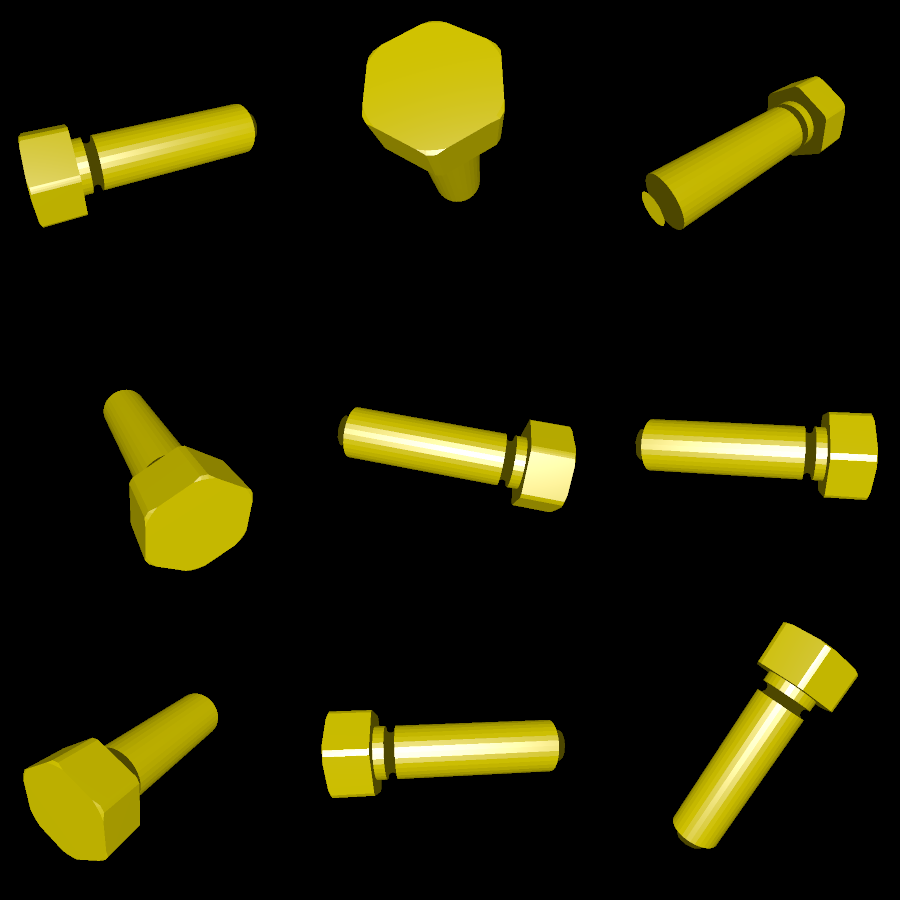
\includegraphics[width=0.3\linewidth]{figures/part_02_chamfer_remaining.png}
    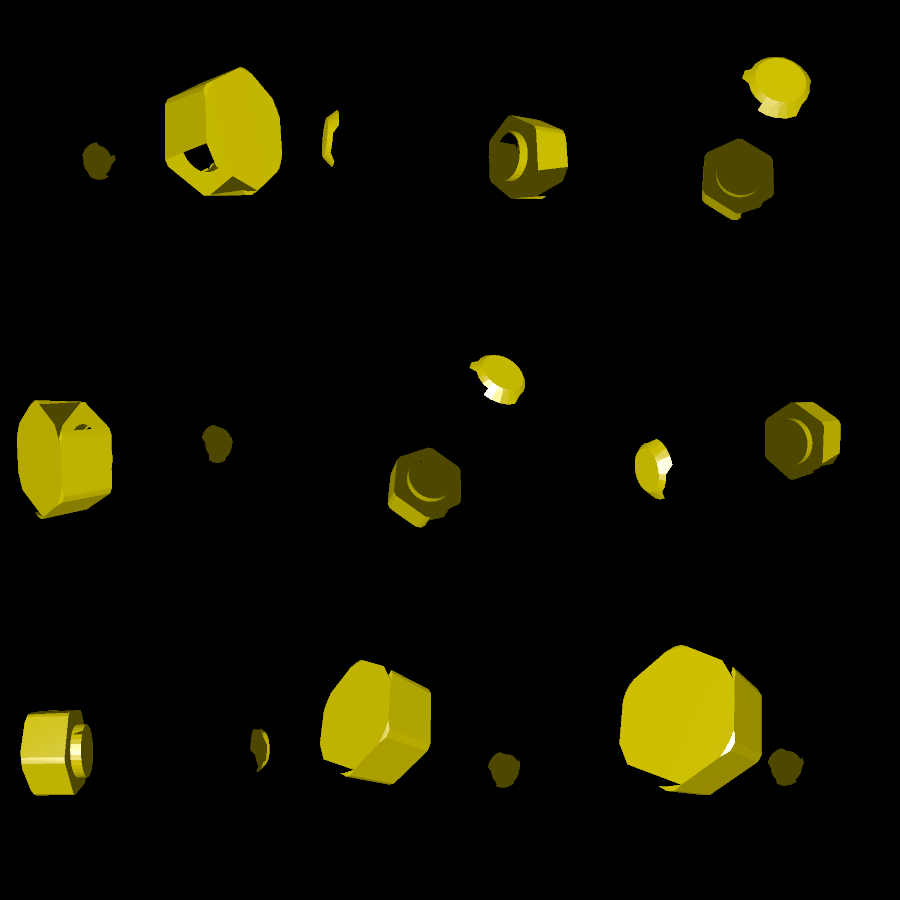
\includegraphics[width=0.3\linewidth]{figures/part_02_bossextrusion_detected.png}
    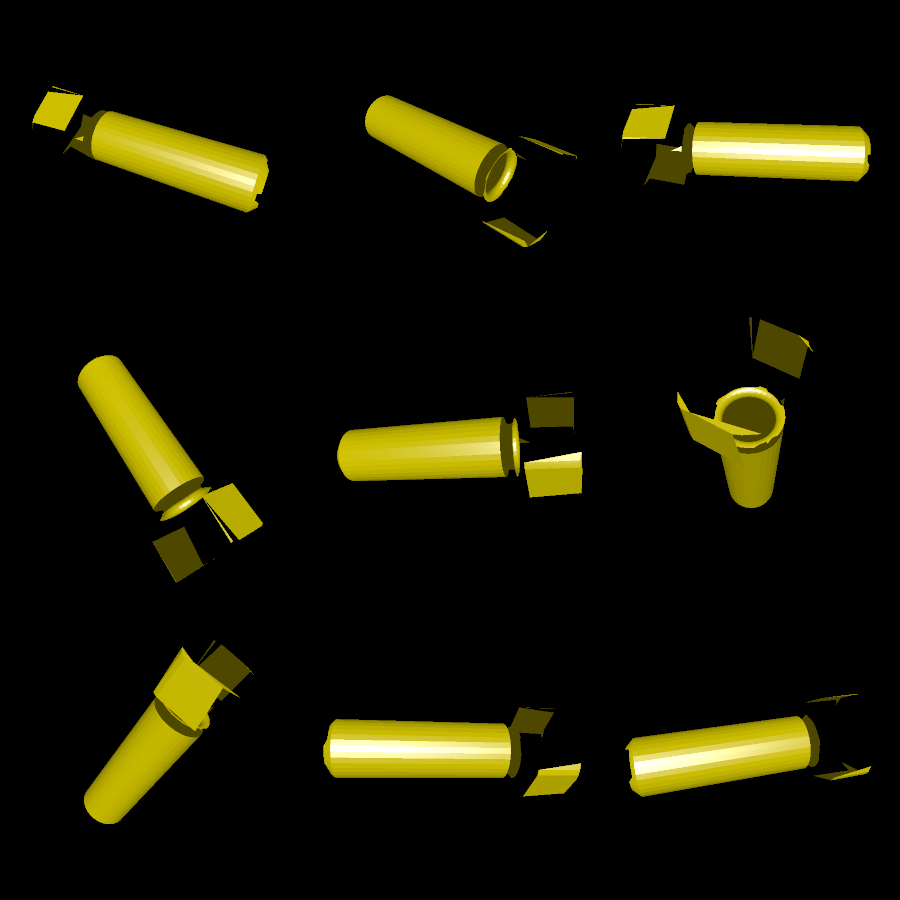
\includegraphics[width=0.3\linewidth]{figures/part_02_bossextrusion_remaining.png}
    \caption{Пример работы модуля на детали «Деталь 02», слева направо, сверху вниз: 1) исходная модель, 2) обнаруженная часть (fillet), 3) оставшаяся геометрия (fillet), 4) обнаруженная часть (cutExtrusion), 5) оставшаяся геометрия (cutExtrusion), 6) обнаруженная часть (chamfer), 7) оставшаяся геометрия (chamfer), 8) обнаруженная часть (bossExtrusion), 9) оставшаяся геометрия (bossExtrusion)}
    \label{fig:part-02}
\end{figure}

\subsection{Деталь 03}

\begin{itemize}
    \item \textbf{Операции исходного построения:} bossRotated, chamfer.
    \item \textbf{Использованные конфигурации нейронных сетей:} классификация - B, сегментация - E.
    \item \textbf{Результат классификации:} fillet - 0.852\%, cutExtrusion - 0.497\%, chamfer - 0.935\%.
\end{itemize}

Результаты сегментации представлены на рисунке \ref{fig:part-03}.

\begin{figure}[h]
    \centering
    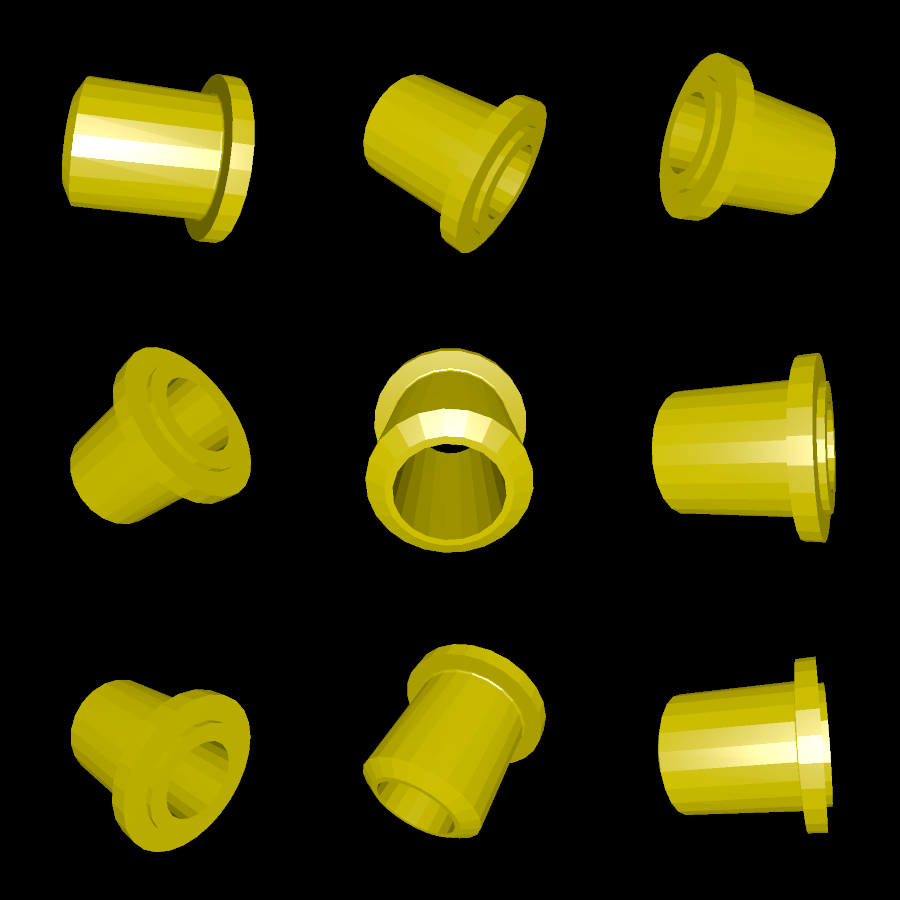
\includegraphics[width=0.3\linewidth]{figures/part_03_original.png}
    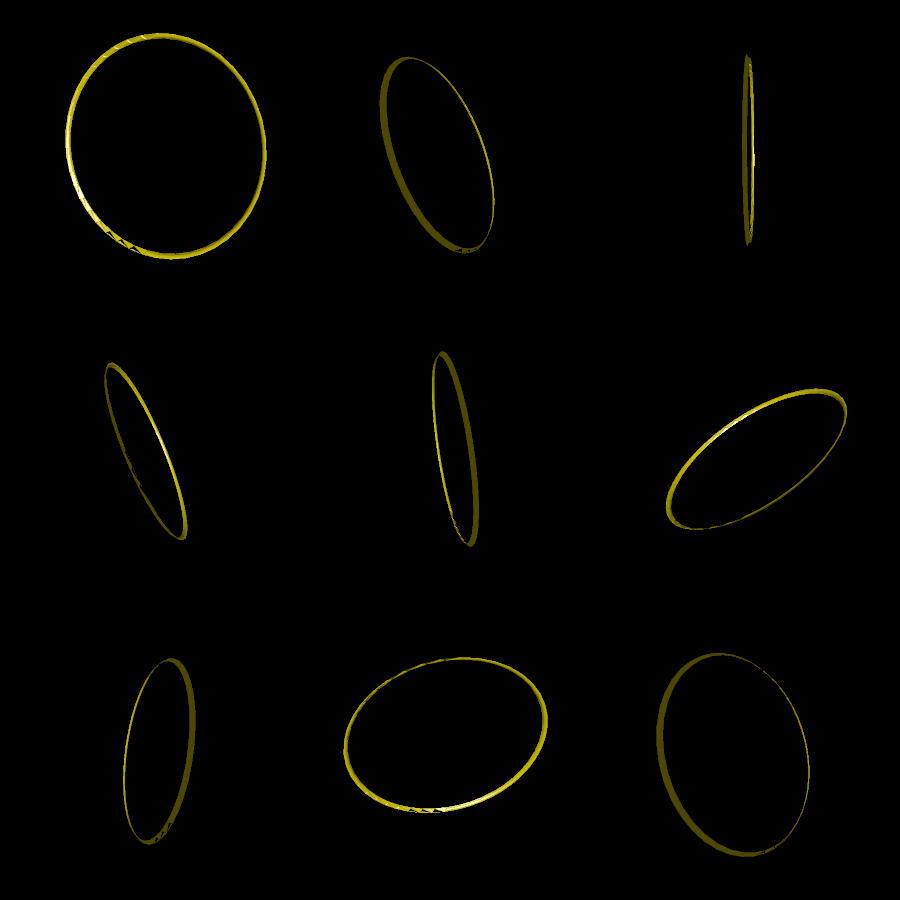
\includegraphics[width=0.3\linewidth]{figures/part_03_fillet_detected.png}
    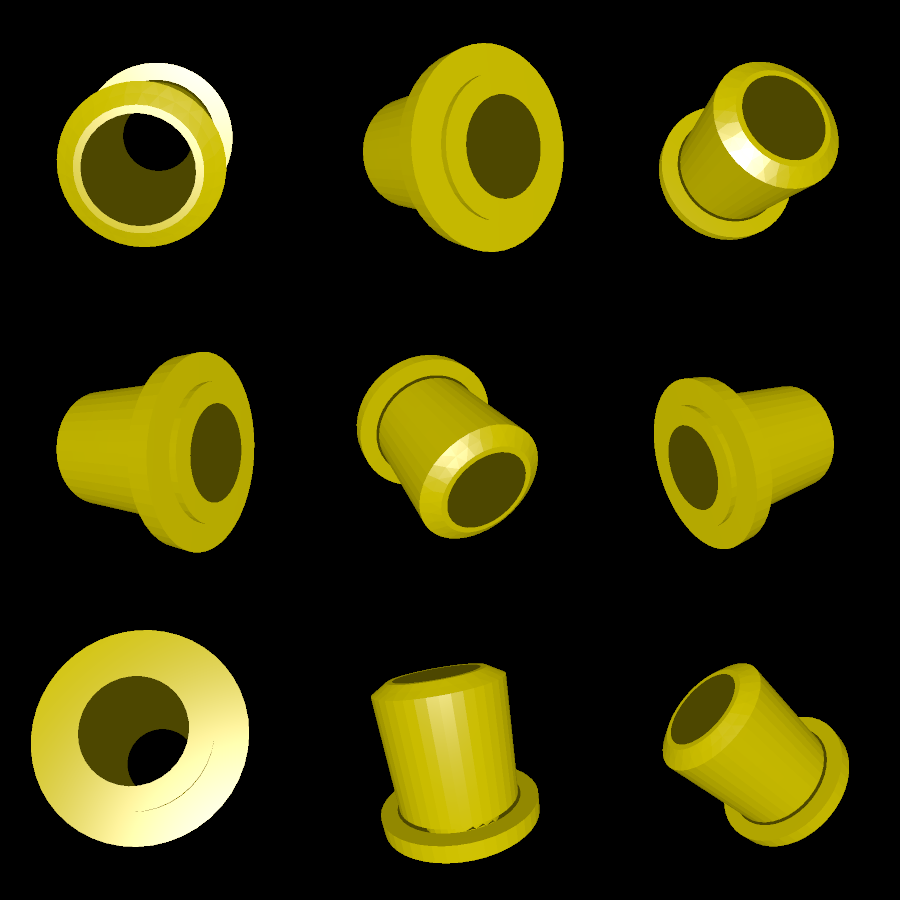
\includegraphics[width=0.3\linewidth]{figures/part_03_fillet_remaining.png} \\
    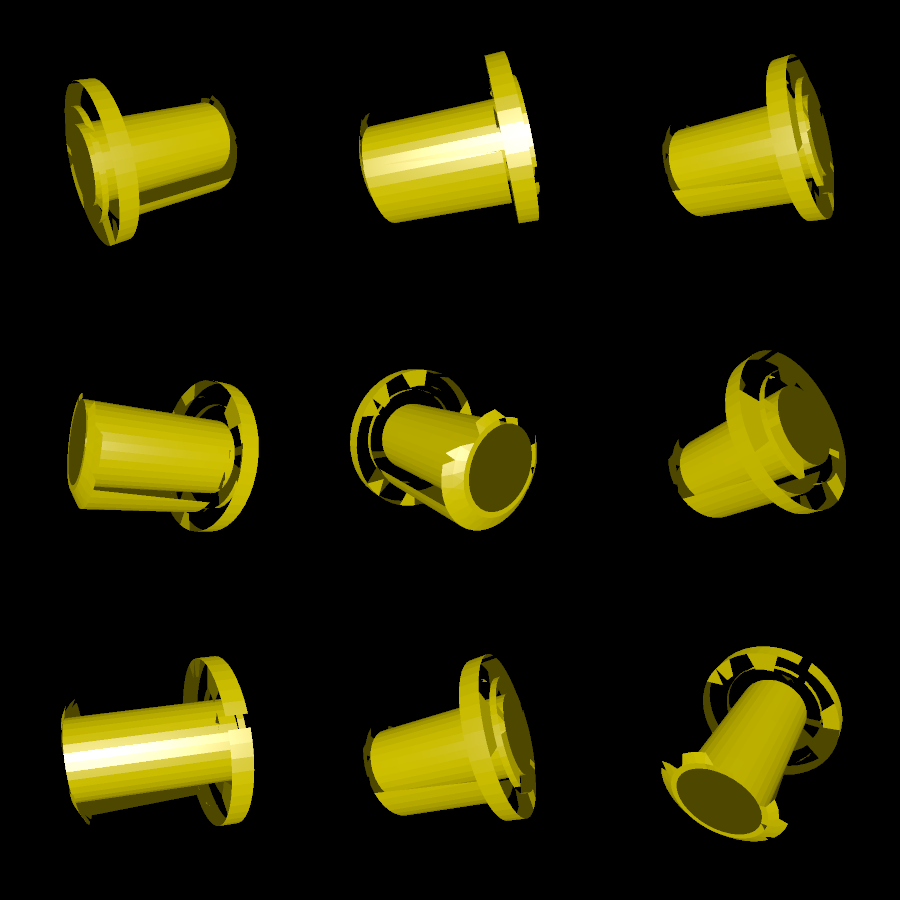
\includegraphics[width=0.3\linewidth]{figures/part_03_cutextrusion_detected.png}
    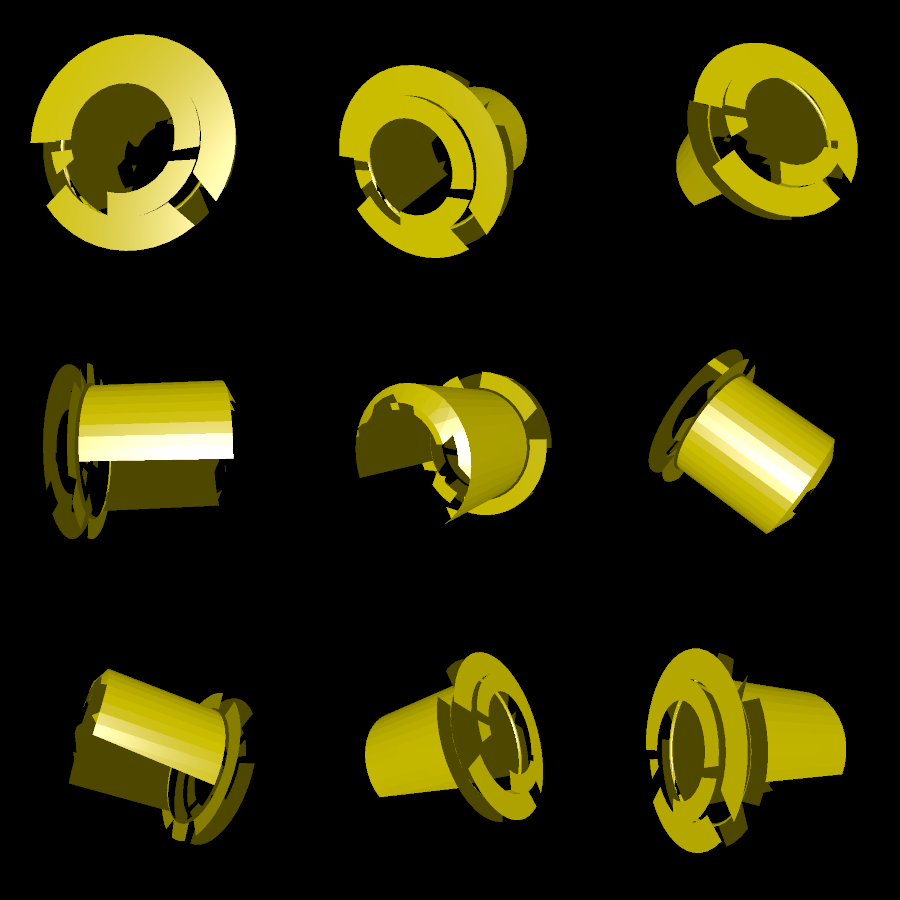
\includegraphics[width=0.3\linewidth]{figures/part_03_cutextrusion_remaining.png}
    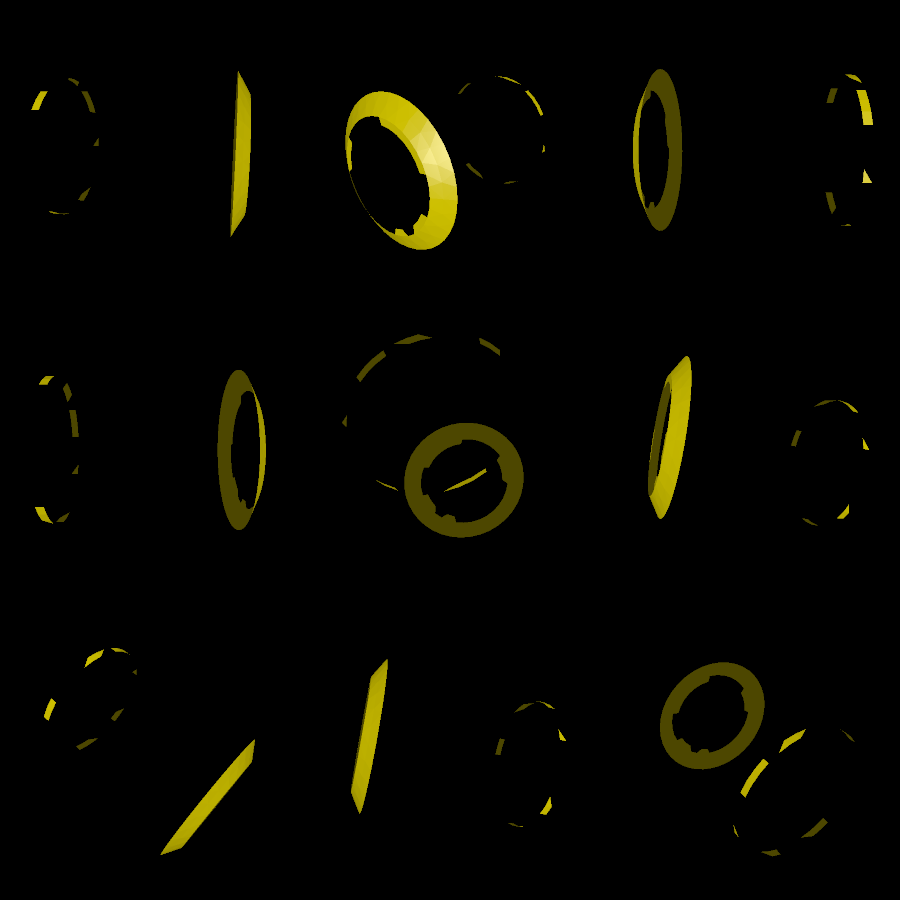
\includegraphics[width=0.3\linewidth]{figures/part_03_chamfer_detected.png} \\
    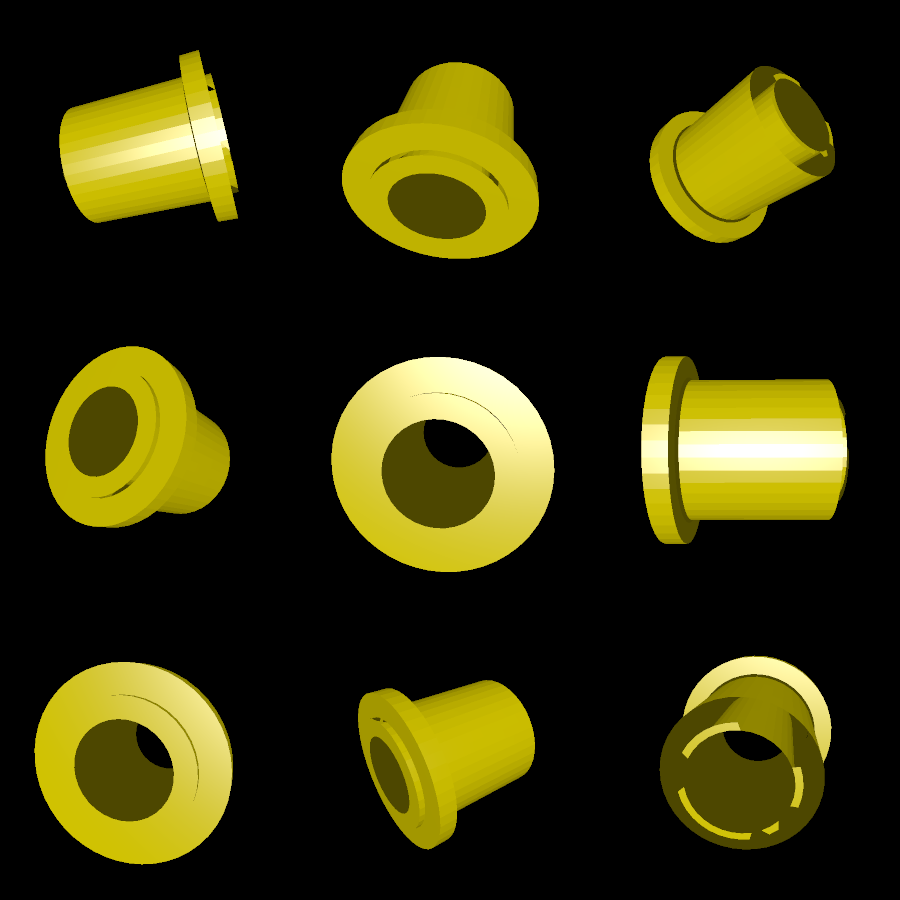
\includegraphics[width=0.3\linewidth]{figures/part_03_chamfer_remaining.png}
    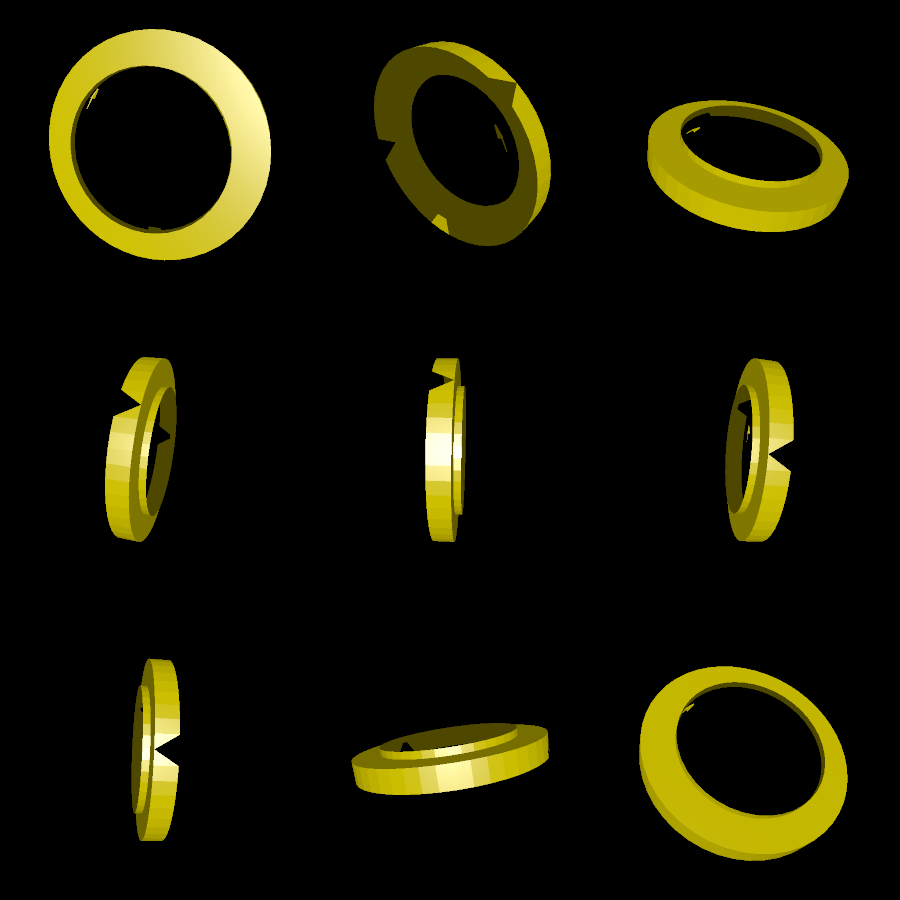
\includegraphics[width=0.3\linewidth]{figures/part_03_bossextrusion_detected.png}
    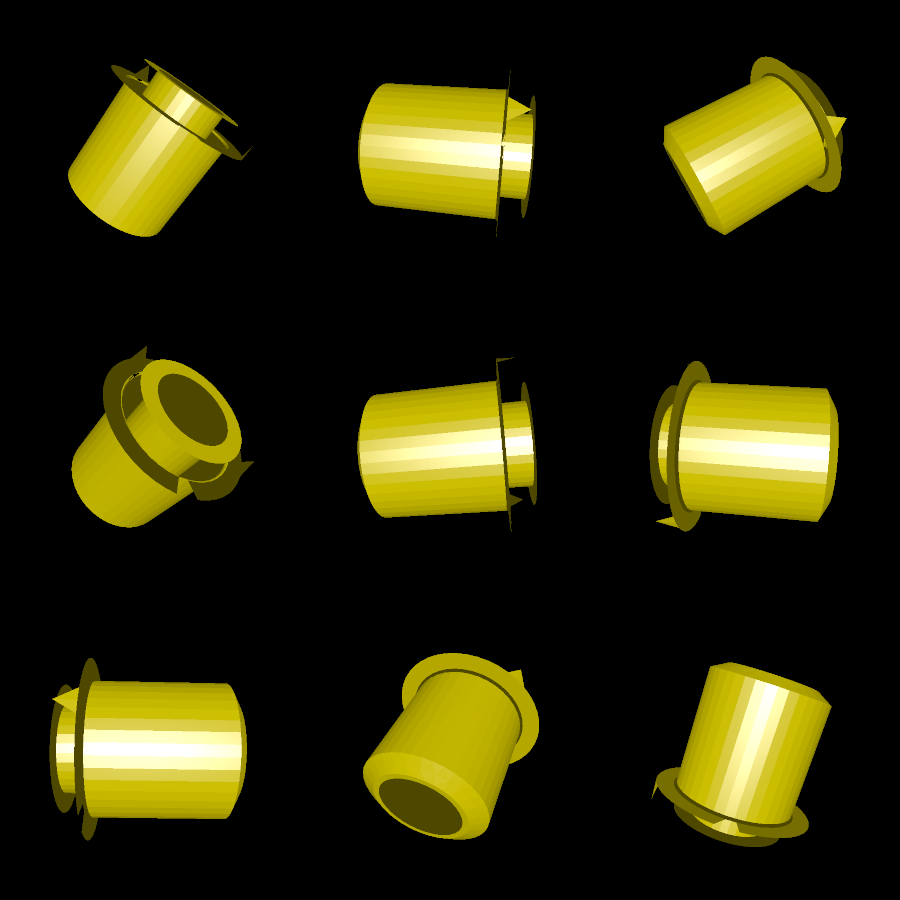
\includegraphics[width=0.3\linewidth]{figures/part_03_bossextrusion_remaining.png}
    \caption{Пример работы модуля на детали «Деталь 03», слева направо, сверху вниз: 1) исходная модель, 2) обнаруженная часть (fillet), 3) оставшаяся геометрия (fillet), 4) обнаруженная часть (cutExtrusion), 5) оставшаяся геометрия (cutExtrusion), 6) обнаруженная часть (chamfer), 7) оставшаяся геометрия (chamfer), 8) обнаруженная часть (bossExtrusion), 9) оставшаяся геометрия (bossExtrusion)}
    \label{fig:part-03}
\end{figure}

\subsection{Деталь 04}

\begin{itemize}
    \item \textbf{Операции исходного построения:} bossRotated, fillet, fillet, chamfer, chamfer, chamfer, cutExtrusion, cutExtrusion, cutExtrusion, cutExtrusion, cutExtrusion, cutExtrusion, chamfer, chamfer, fillet.
    \item \textbf{Использованные конфигурации нейронных сетей:} классификация - B, сегментация - C.
    \item \textbf{Результат классификации:} fillet - 0.985\%, cutExtrusion - 0.546\%, chamfer - 0.978\%.
\end{itemize}

Результаты сегментации представлены на рисунке \ref{fig:part-04}.

\begin{figure}[h]
    \centering
    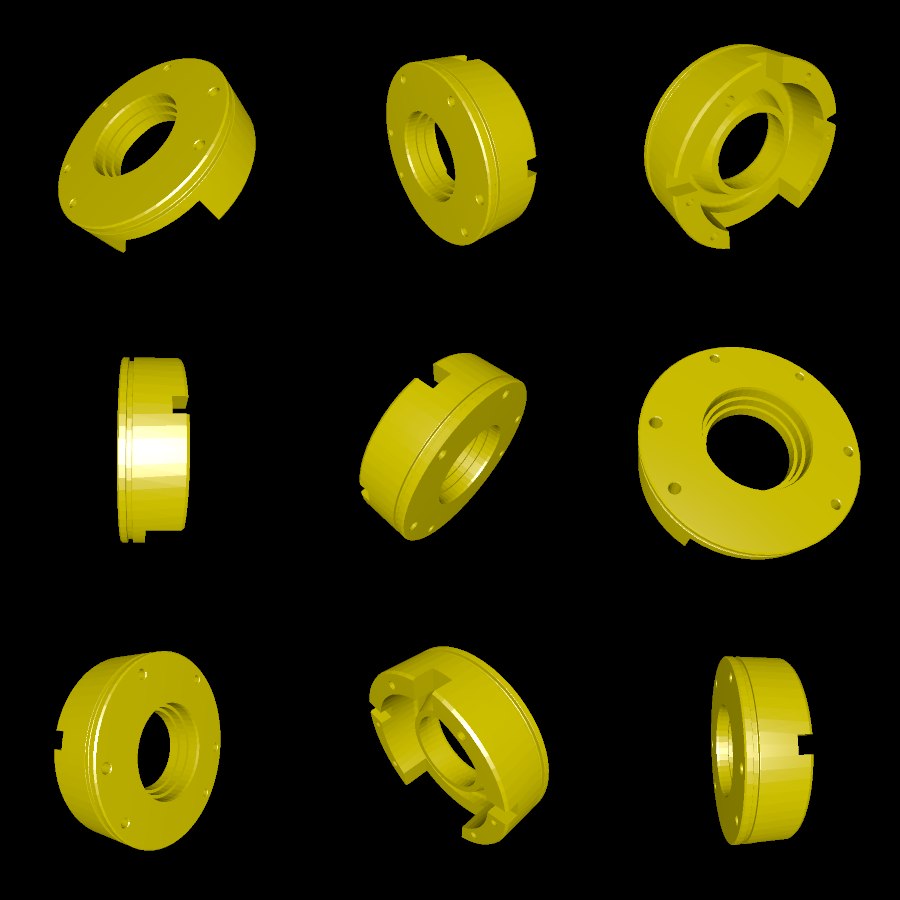
\includegraphics[width=0.3\linewidth]{figures/part_04_original.png}
    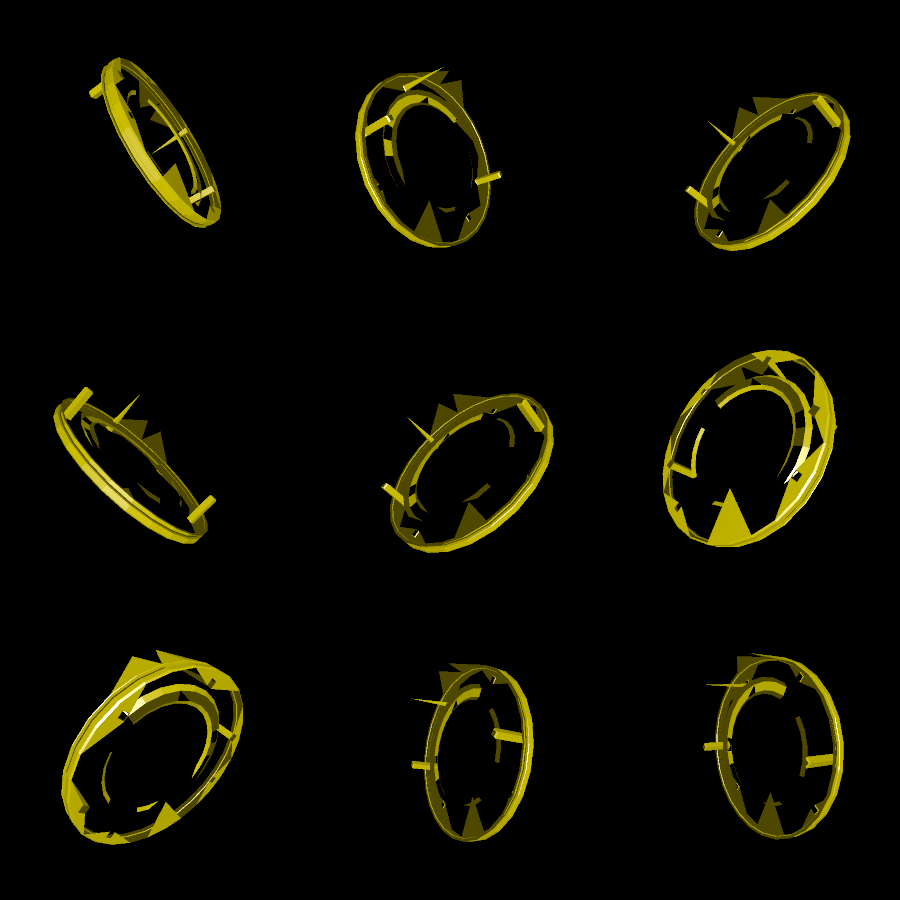
\includegraphics[width=0.3\linewidth]{figures/part_04_fillet_detected.png}
    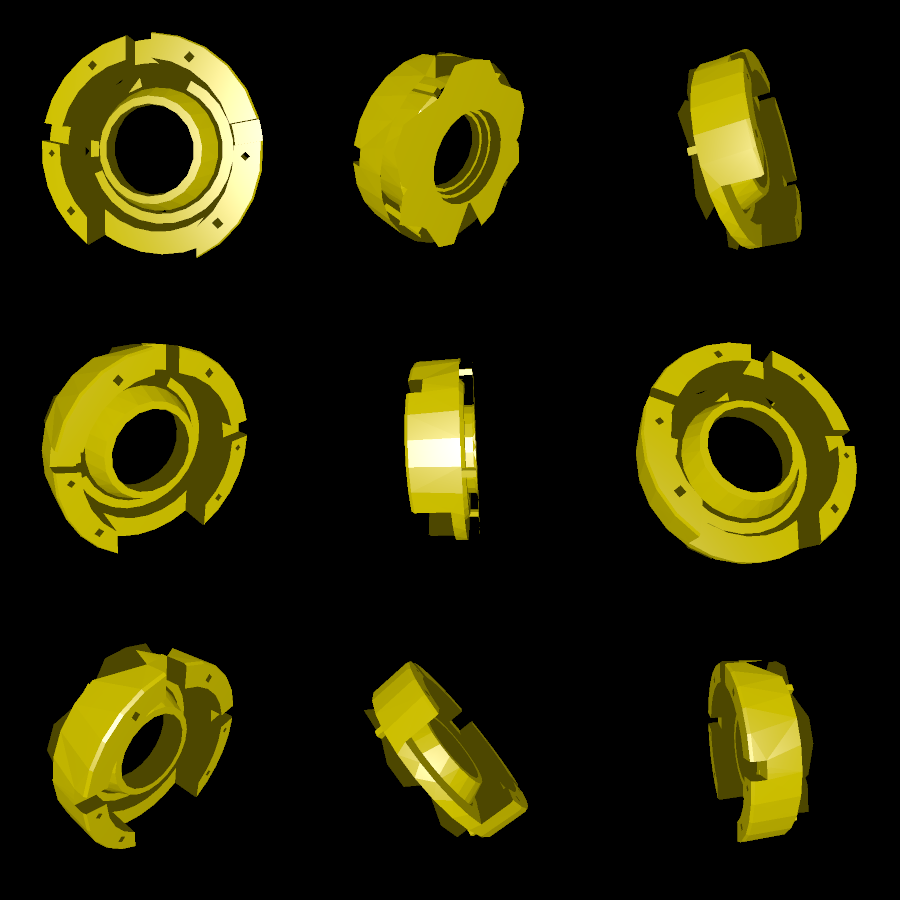
\includegraphics[width=0.3\linewidth]{figures/part_04_fillet_remaining.png} \\
    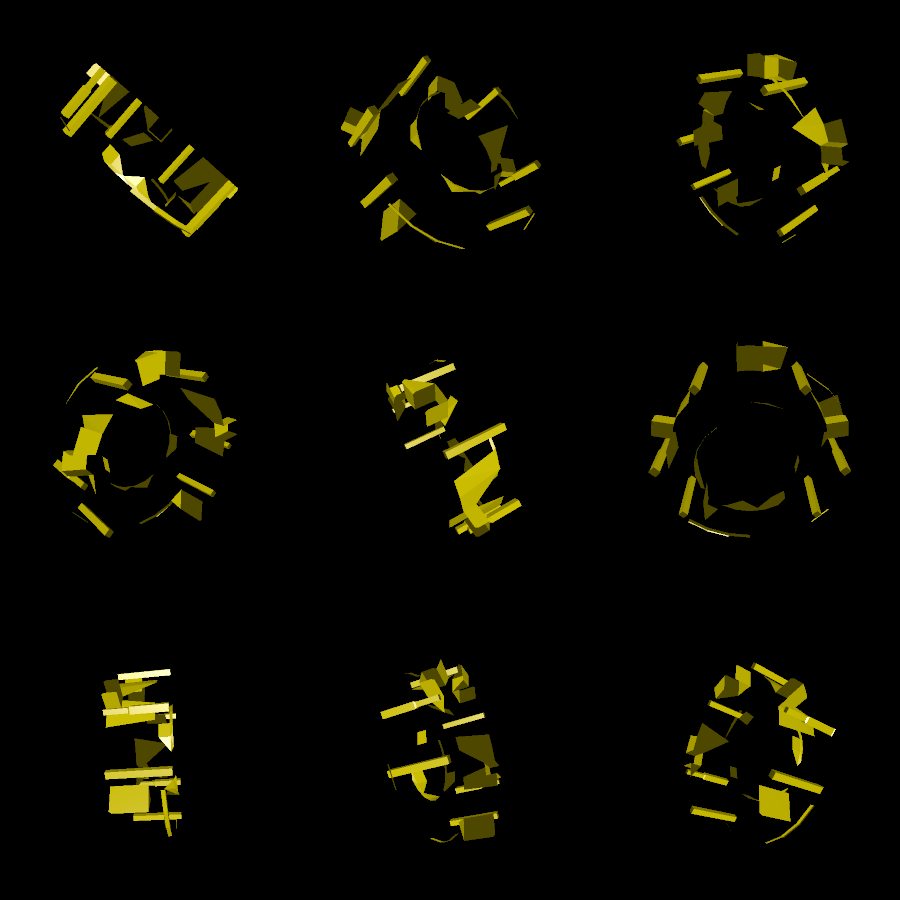
\includegraphics[width=0.3\linewidth]{figures/part_04_cutextrusion_detected.png}
    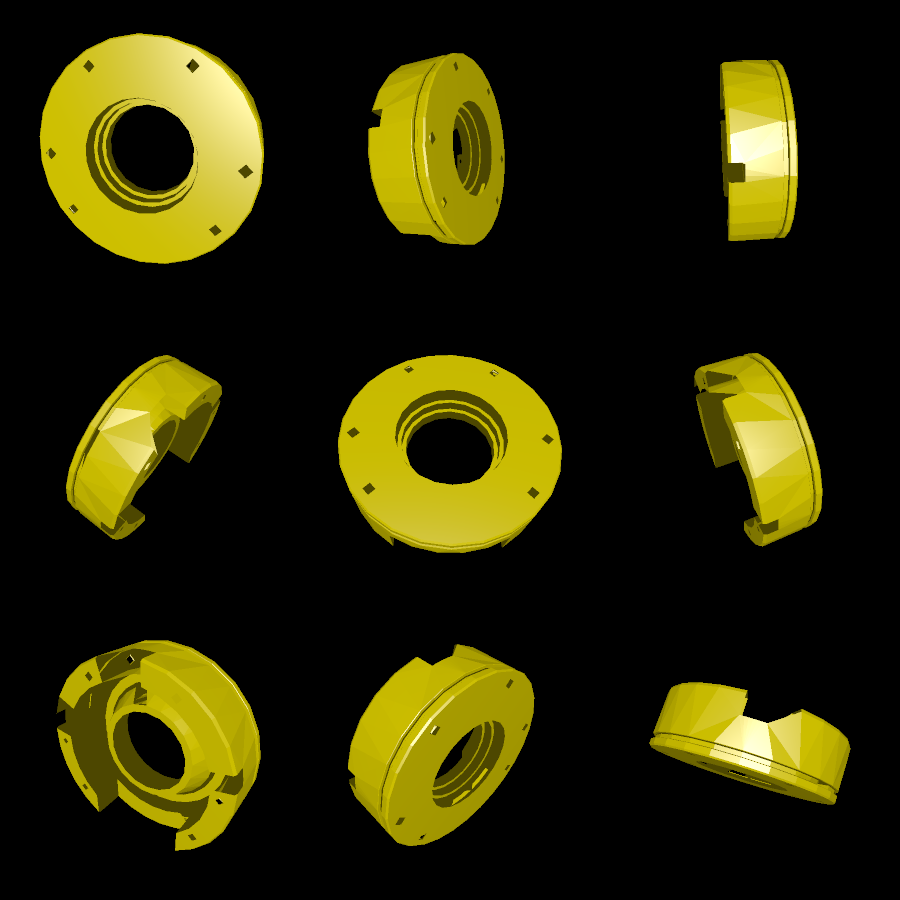
\includegraphics[width=0.3\linewidth]{figures/part_04_cutextrusion_remaining.png}
    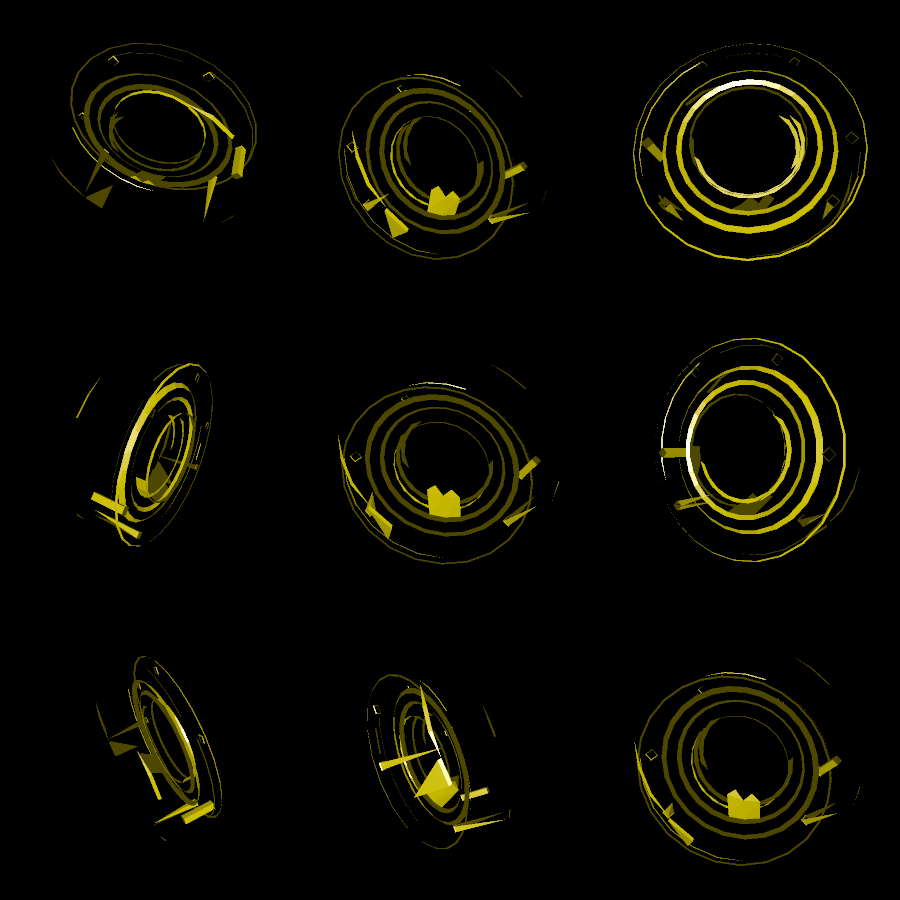
\includegraphics[width=0.3\linewidth]{figures/part_04_chamfer_detected.png} \\
    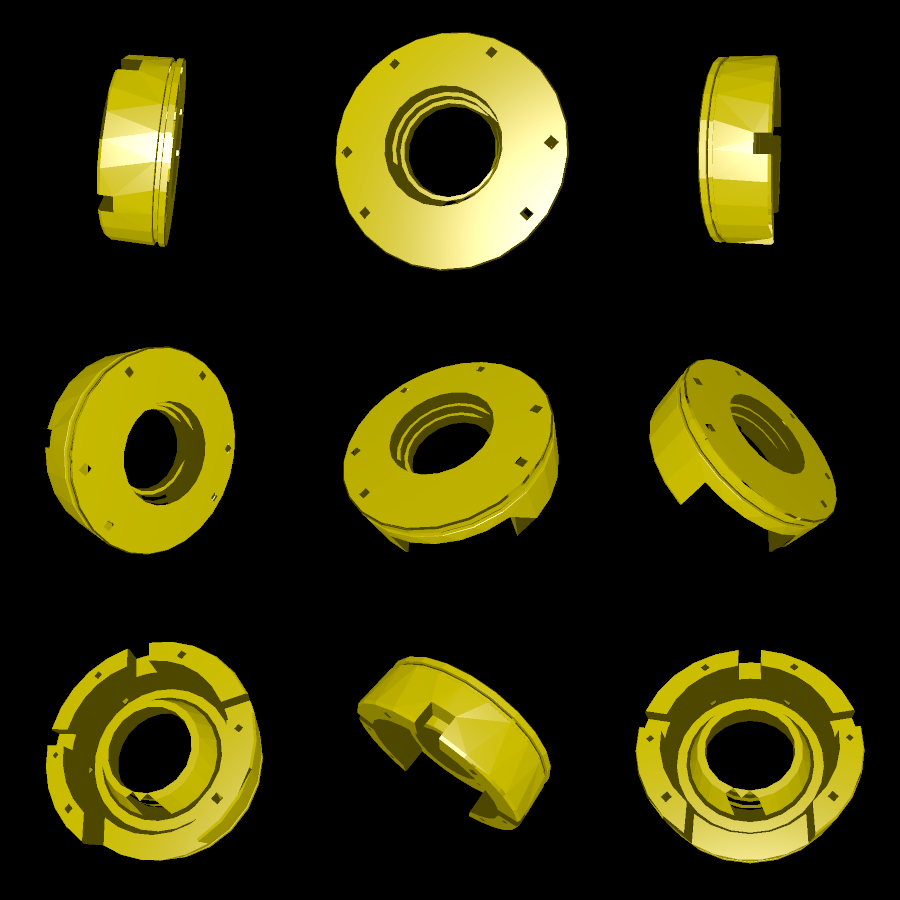
\includegraphics[width=0.3\linewidth]{figures/part_04_chamfer_remaining.png}
    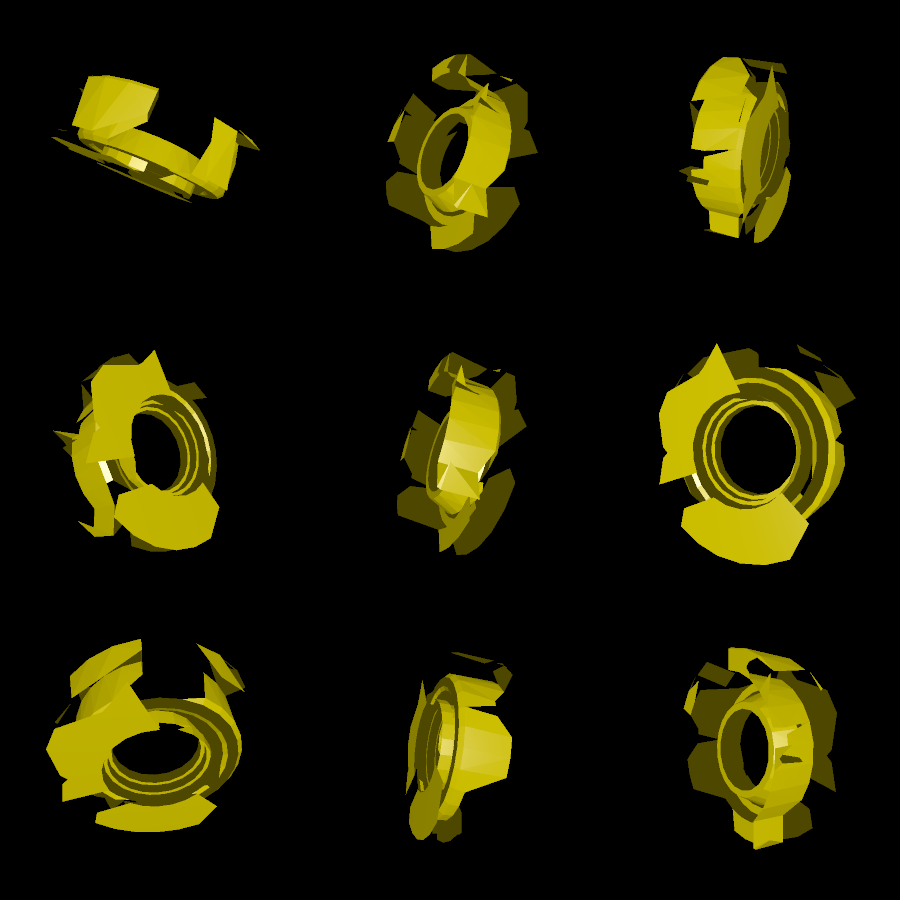
\includegraphics[width=0.3\linewidth]{figures/part_04_bossextrusion_detected.png}
    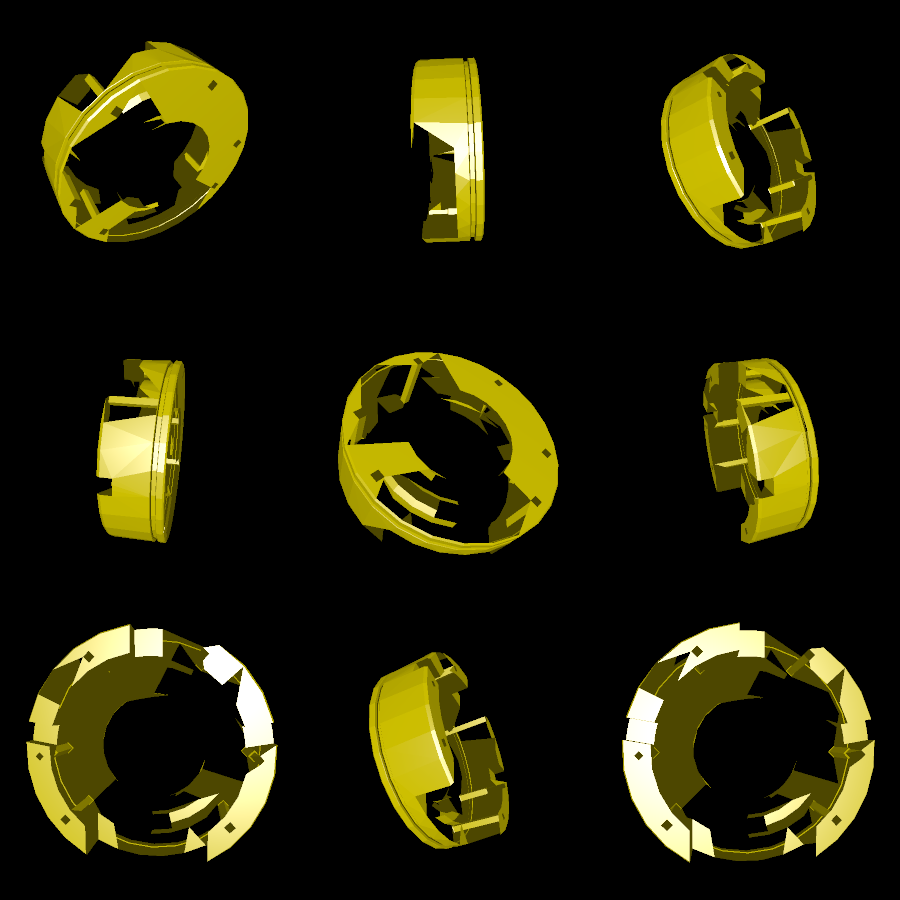
\includegraphics[width=0.3\linewidth]{figures/part_04_bossextrusion_remaining.png}
    \caption{Пример работы модуля на детали «Деталь 04», слева направо, сверху вниз: 1) исходная модель, 2) обнаруженная часть (fillet), 3) оставшаяся геометрия (fillet), 4) обнаруженная часть (cutExtrusion), 5) оставшаяся геометрия (cutExtrusion), 6) обнаруженная часть (chamfer), 7) оставшаяся геометрия (chamfer), 8) обнаруженная часть (bossExtrusion), 9) оставшаяся геометрия (bossExtrusion)}
    \label{fig:part-04}
\end{figure}

\subsection{Деталь 05}

\begin{itemize}
    \item \textbf{Операции исходного построения:} bossExtrusion, fillet, chamfer, bossExtrusion, fillet, bossExtrusion.
    \item \textbf{Использованные конфигурации нейронных сетей:} классификация - B, сегментация - C.
    \item \textbf{Результат классификации:} fillet - 0.979\%, cutExtrusion - 0.355\%, chamfer - 0.444\%.
\end{itemize}

Результаты сегментации представлены на рисунке \ref{fig:part-05}.

\begin{figure}[h]
    \centering
    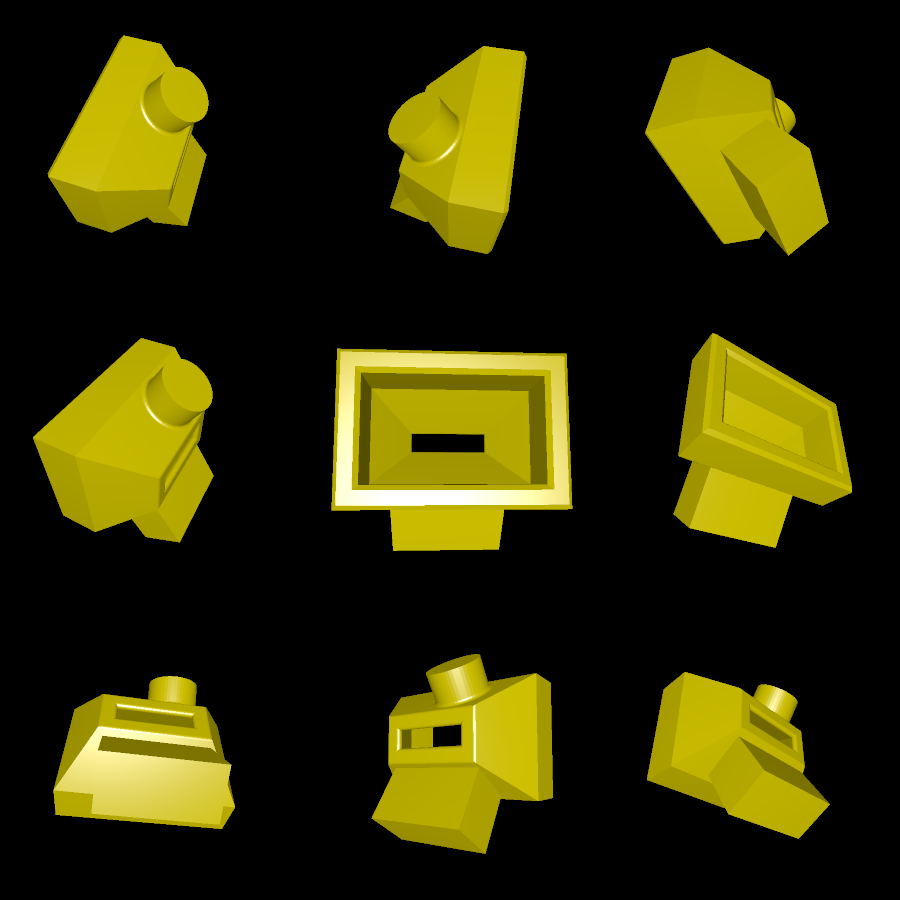
\includegraphics[width=0.3\linewidth]{figures/part_05_original.png}
    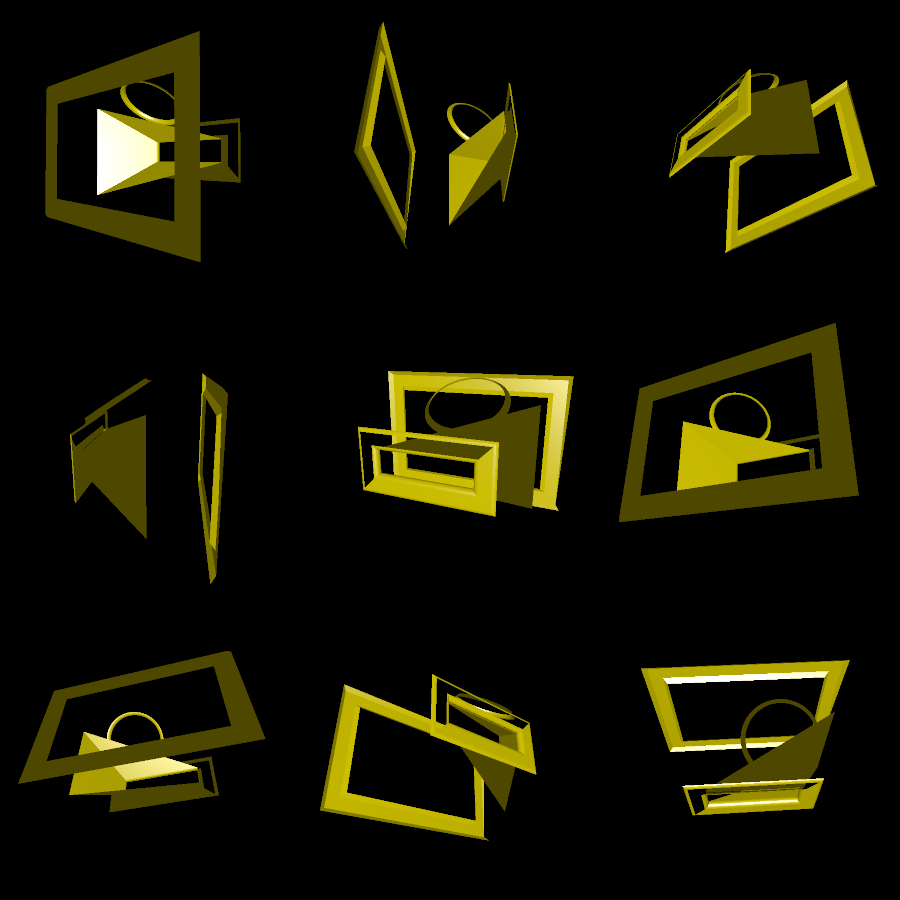
\includegraphics[width=0.3\linewidth]{figures/part_05_fillet_detected.png}
    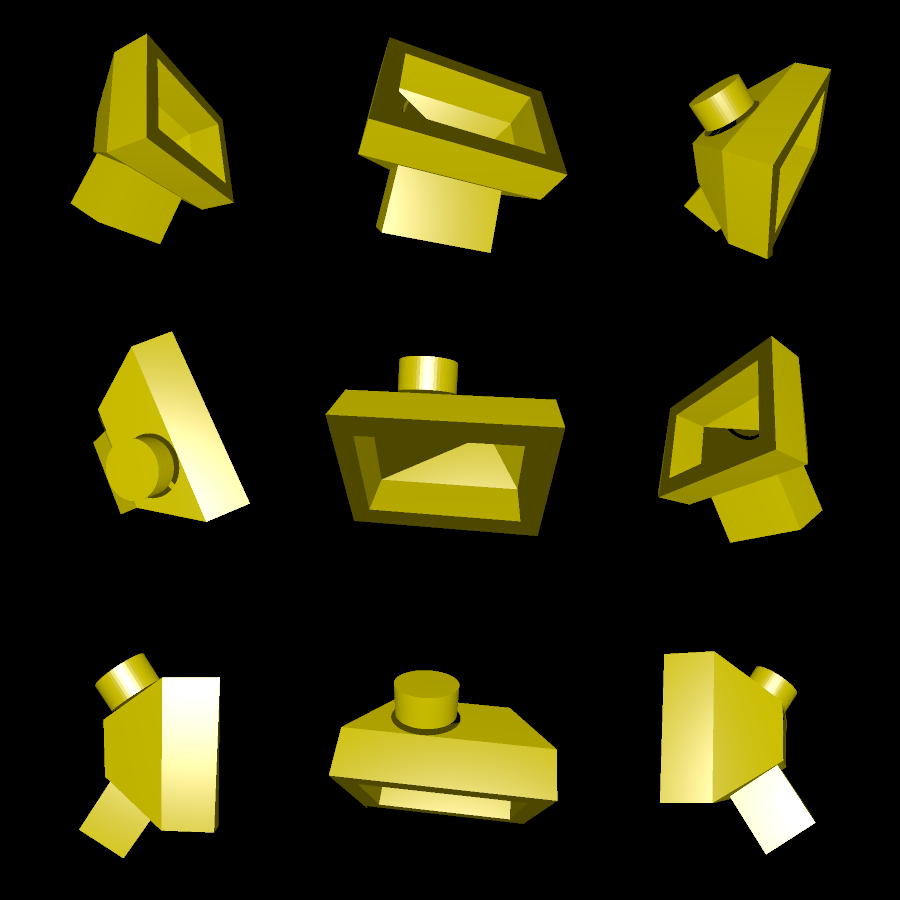
\includegraphics[width=0.3\linewidth]{figures/part_05_fillet_remaining.png} \\
    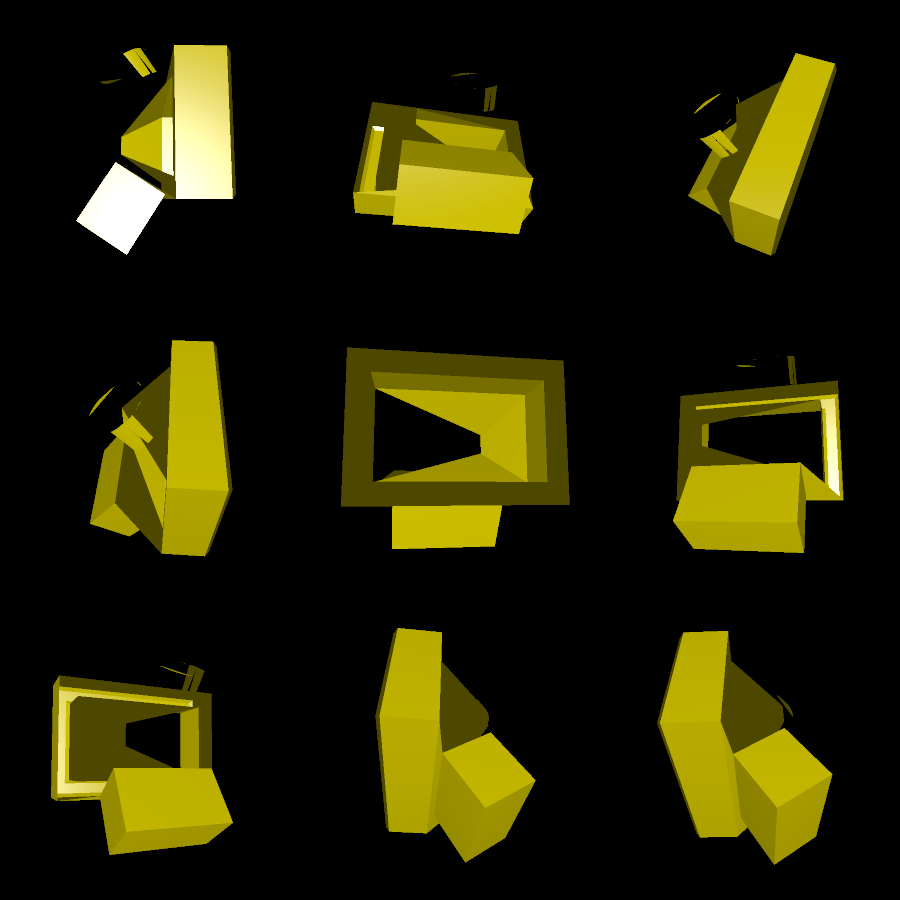
\includegraphics[width=0.3\linewidth]{figures/part_05_cutextrusion_detected.png}
    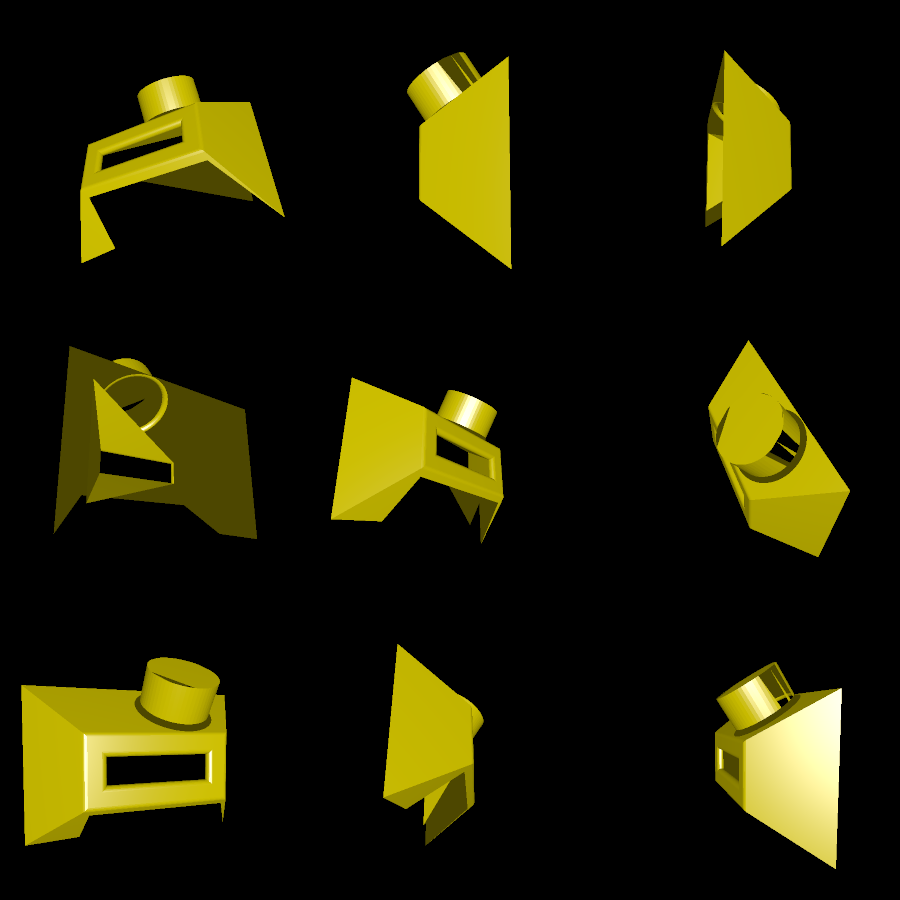
\includegraphics[width=0.3\linewidth]{figures/part_05_cutextrusion_remaining.png}
    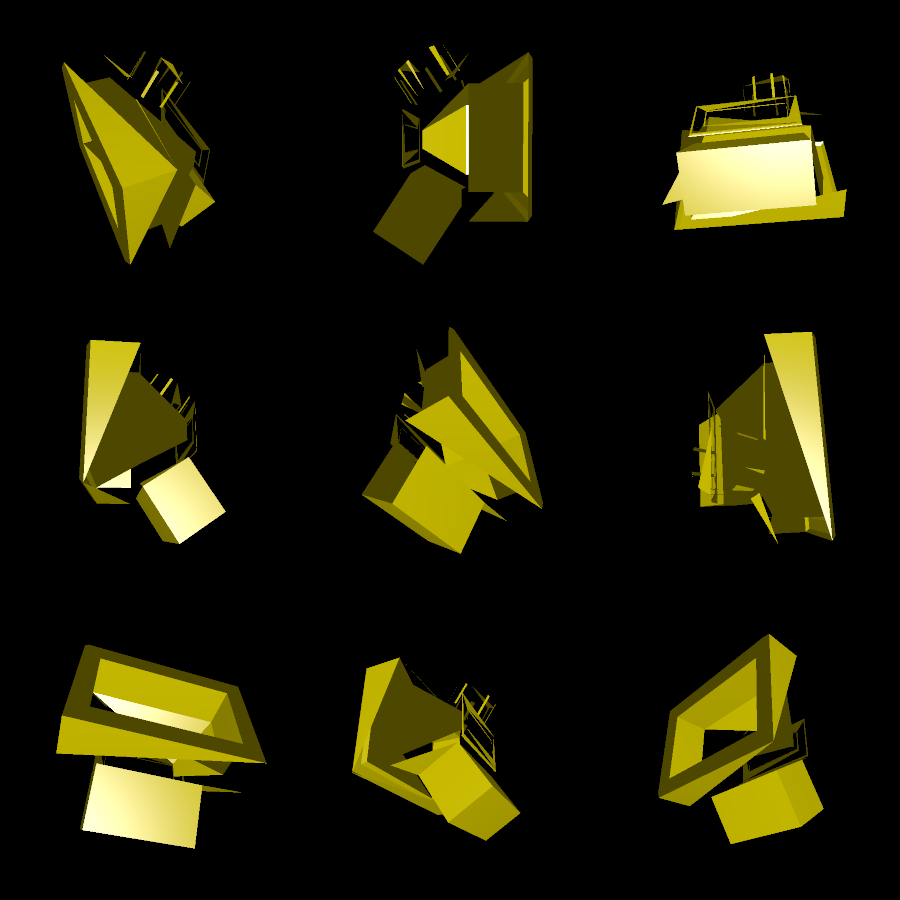
\includegraphics[width=0.3\linewidth]{figures/part_05_chamfer_detected.png} \\
    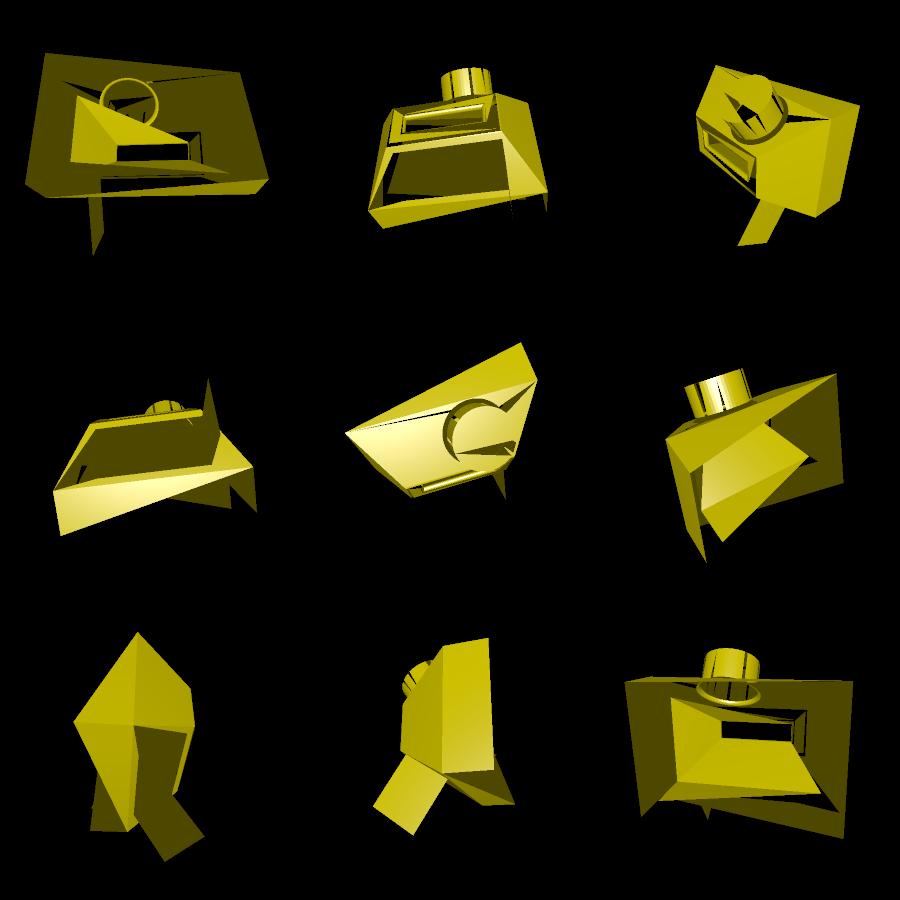
\includegraphics[width=0.3\linewidth]{figures/part_05_chamfer_remaining.png}
    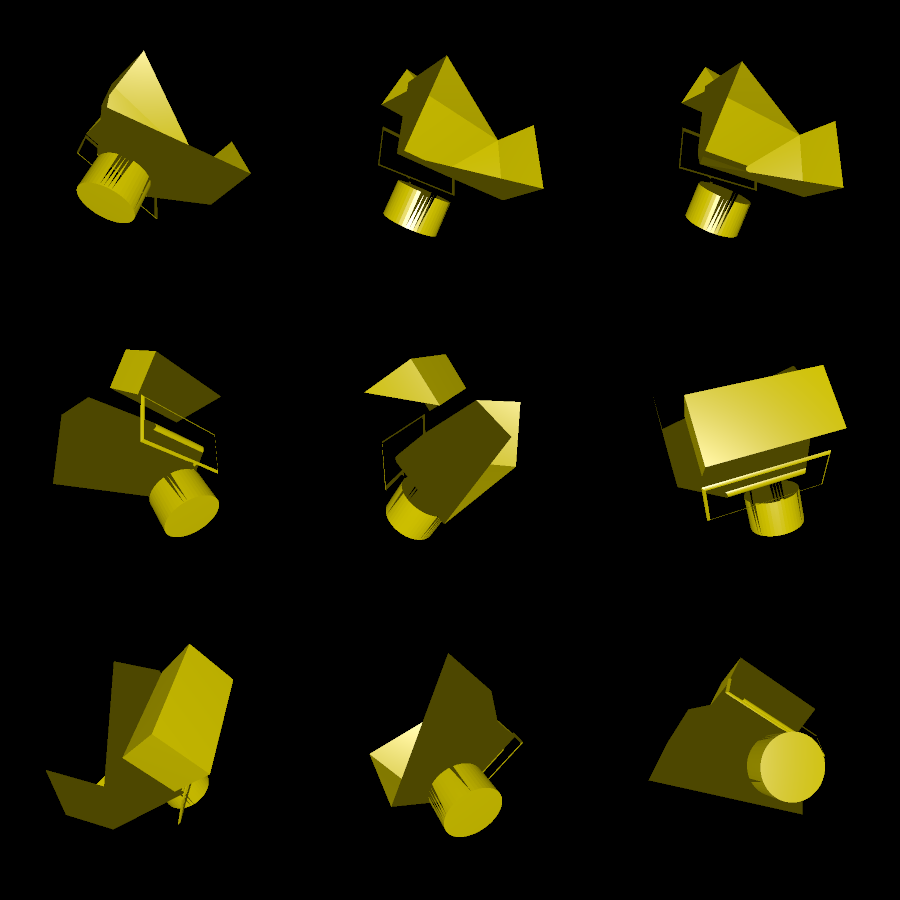
\includegraphics[width=0.3\linewidth]{figures/part_05_bossextrusion_detected.png}
    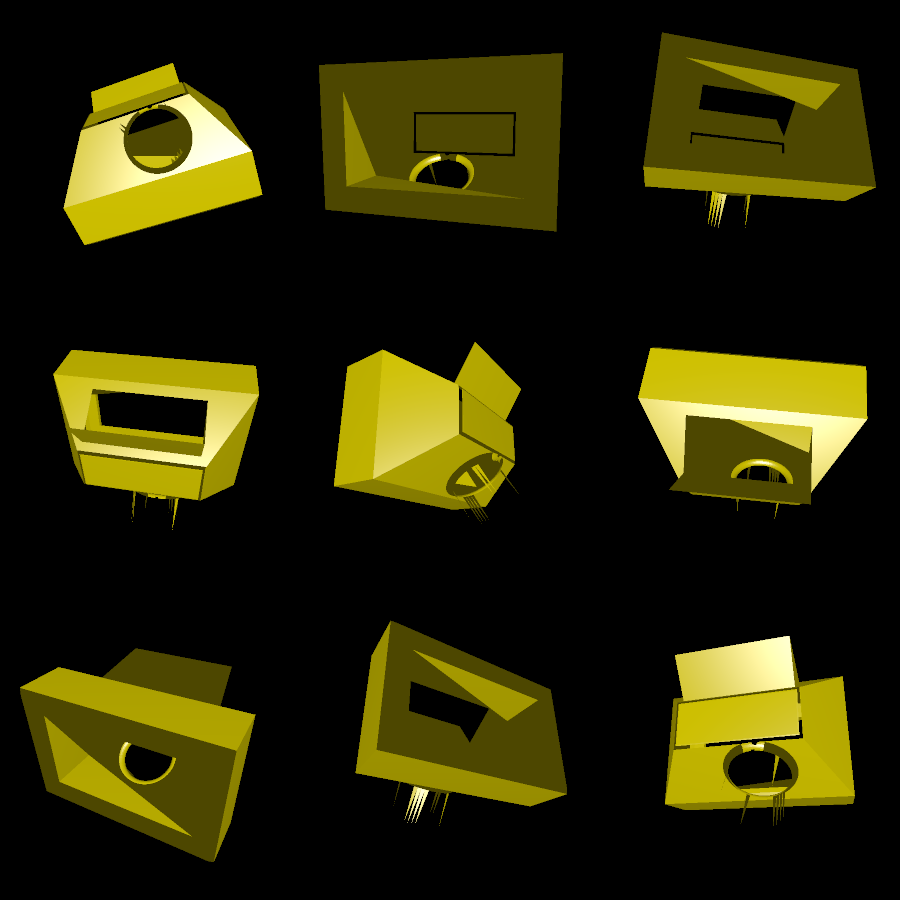
\includegraphics[width=0.3\linewidth]{figures/part_05_bossextrusion_remaining.png}
    \caption{Пример работы модуля на детали «Деталь 05», слева направо, сверху вниз: 1) исходная модель, 2) обнаруженная часть (fillet), 3) оставшаяся геометрия (fillet), 4) обнаруженная часть (cutExtrusion), 5) оставшаяся геометрия (cutExtrusion), 6) обнаруженная часть (chamfer), 7) оставшаяся геометрия (chamfer), 8) обнаруженная часть (bossExtrusion), 9) оставшаяся геометрия (bossExtrusion)}
    \label{fig:part-05}
\end{figure}

